\documentclass[8pt,landscape,a4paper]{extarticle}
\usepackage[landscape]{geometry}
\usepackage{graphicx}
\graphicspath{ {images/} }
\usepackage{amssymb,amsmath,amsthm,amsfonts,mathtools}
\usepackage{multicol,multirow}
\usepackage{enumitem}
\usepackage[explicit]{titlesec}
\usepackage[many]{tcolorbox}
\usepackage{wallpaper}
\usepackage{fancyhdr} 
\usepackage{tikz}
\usepackage{array}
\usepackage{tabularx}
\usepackage{makecell}
\usepackage{nicefrac,xfrac}
\usepackage{bm}
\usepackage{wrapfig}
\usepackage{caption}
\usepackage{hyperref}
% \captionsetup[figure]{name=Fig.}

\geometry{top=16pt,left=15pt,right=15pt,bottom=15pt, % margins
          includehead=false,          % header out of text body
          headheight =10pt,           % header height
          headsep = 4pt,              % header seperation
          footskip=10pt}
\linespread{.5}
\setlist{nosep}

% Define header
\fancyhf{}
\pagestyle{fancy}
\lhead{\textbf{Model Predictive Control FS26}}
\rhead{\texttt{A. Bernasconi, abernasconi@student.ethz.ch | F. Frigerio, ffrigerio@student.ethz.ch | M. Dal Bò, mdalbo@student.ethz.ch}}
\cfoot{\textit{Page \thepage}}
\setcounter{secnumdepth}{0}

% Define new length
\newlength{\titlesep}
\setlength{\titlesep}{3pt}

% Define whitespace command
\newcommand{\whitespace}[1][4pt]{\titleline[c]{\color{white}\rule{2\titlesep+\linewidth}{#1}}}

% Define section
\titleformat{\section}[display]{\large\bfseries}{}{0pt}{%
	\vspace{4pt+\baselineskip+5pt}	% Cancels second vspace
	\vspace*{-4pt-\baselineskip-5pt} % if not at beginning of page
	\begin{tcolorbox}[
		arc=0pt,
		boxsep=0pt,
		boxrule=0pt,
		toprule=4pt,
		top=4pt,
		bottom=4pt,
		middle=0pt,
		left=\titlesep,
		right=\titlesep,
		nobeforeafter,
		before skip = 0pt,
		leftright skip=-\titlesep,
		after skip=-\parskip-\baselineskip-2pt,
		colframe=white,
		colback=white!30!black
		]\color{white}#1
	\end{tcolorbox}%
}

\makeatother

% Define  subsection
\titleformat{\subsection}[display]{\large\bfseries}{}{0pt}{%
	\vspace{2pt+\baselineskip+5pt}	% Cancels second vspace
	\vspace*{-2pt-\baselineskip-5pt} % if not at beginning of page
	\begin{tcolorbox}[
		arc=0pt,
		boxsep=0pt,
		boxrule=0pt,
		toprule=2pt,
		top=3pt,
		bottom=3pt,
		middle=0pt,
		left=\titlesep,
		right=\titlesep,
		nobeforeafter,
		before skip = 0pt,
		leftright skip=-\titlesep,
        after skip=-\parskip-\baselineskip-1pt,
		colframe=white,
		colback=white!60!black
		]#1
	\end{tcolorbox}%
}
      
% Define subsubsection
\titleformat{\subsubsection}[display]{\normalsize\bfseries}{}{0pt}{%
	\begin{tcolorbox}[
		arc=0pt,
		boxsep=0pt,
		boxrule=0pt,
		top=3pt,
		bottom=3pt,
		middle=0pt,
		left=\titlesep,
		right=\titlesep,
		nobeforeafter,
		leftright skip=-\titlesep,
        after skip=-\parskip-\baselineskip-1pt,
		colframe=white,
		colback=white!85!black
		]#1
	\end{tcolorbox}%
}

% Define spacings
\titlespacing{\section}
  {0pt}{2pt}{0pt}
\titlespacing{\subsection}
  {0pt}{.5pt}{0pt}
\titlespacing{\subsubsection}
  {0pt}{0pt}{0pt}

% Set sans-serif
\renewcommand{\familydefault}{\sfdefault}

% Define column-sep
\raggedcolumns
\setlength{\columnsep}{17pt}

% Renew sizes
\renewcommand{\large}{\normalsize}
\renewcommand{\normalsize}{\small}
\renewcommand{\small}{\footnotesize}
% Make arrow symbols safe to use in text mode too
\let\originalrightarrow\rightarrow
\renewcommand{\rightarrow}{\ensuremath{\originalrightarrow}}
\let\originalRightarrow\Rightarrow
\renewcommand{\Rightarrow}{\ensuremath{\originalRightarrow}}
\let\originalLeftrightarrow\Leftrightarrow
\renewcommand{\Leftrightarrow}{\ensuremath{\originalLeftrightarrow}}

% Define custom math operators
\DeclareMathOperator*{\argmax}{arg\,max}
\DeclareMathOperator*{\argmin}{arg\,min}
\DeclareMathOperator*{\E}{\mathrm{E}}
\DeclareMathOperator*{\Var}{\mathrm{Var}}

% Define new columntype
\newcolumntype{L}[1]{>{\raggedright\let\newline\\\arraybackslash\hspace{0pt}}m{#1}}
\newcolumntype{C}[1]{>{\centering\let\newline\\\arraybackslash\hspace{0pt}}m{#1}}
\newcolumntype{R}[1]{>{\raggedleft\let\newline\\\arraybackslash\hspace{0pt}}m{#1}}

\tcbset{
  eqbox/.style={
    colback=white!92!black,
    colframe=white!60!black,
    arc=0pt,
    boxrule=0.5pt,
    boxsep=0pt,
    left=1.5mm,
    right=1.5mm,
    top=0.2mm,
    bottom=0.2mm,
    before skip=0pt,
    after skip=0pt,
    before upper={
      \setlength{\abovedisplayskip}{0pt}%
      \setlength{\belowdisplayskip}{0pt}%
      \setlength{\abovedisplayshortskip}{0pt}%
      \setlength{\belowdisplayshortskip}{0pt}%
    }
  }
}


% Begin document
\begin{document}

% Set lengths
\setlength{\parindent}{0pt}
\setlength{\parskip}{1pt}
\setlength{\abovedisplayskip}{0pt}
\setlength{\belowdisplayskip}{0pt}
\setlength{\abovedisplayshortskip}{0pt}
\setlength{\belowdisplayshortskip}{0pt}

\begin{multicols*}{3}
\raggedright

%%%%% Content
\section{Introduction}
\subsubsection{Discretization \& Linearization}
{\small
\noindent
\begin{minipage}[t]{0.32\linewidth}

\textbf{Euler Discretization}\\
\begin{align*}
x(k) &= x^c(t_0 + kT_s)\\
u(k) &= u^c(t_0 + kT_s)\\
A &= \mathbb{I} + T_sA^c\\
B &= T_s B^c\\
C &= C^c\\
D &= D^c
\end{align*}
\end{minipage}%
\hfill
\begin{minipage}[t]{0.32\linewidth}

\textbf{Exact Discretization}\\
\begin{align*}
A &= \exp{(A^c \cdot T_s)}\\
B &= \int^{T_s}_0 \exp{(A^c \cdot \tau)}\, d\tau\, B^c\\
C &= C^c\\
D &= D^c
\end{align*}
If $A^c$ invertible:\\
$B = (A^c)^{-1}(A-\mathbb{I})B^c$
\end{minipage}%
\hfill
\begin{minipage}[t]{0.32\linewidth}
\textbf{Linearization (Taylor)}\\
Around $\bar{x},\bar{u}$ (first order):\\
\[
f(\bar{x}) + \frac{\partial f}{\partial x^\top}\Big|_{\bar{x}} \cdot (x-\bar{x})
\]

\vspace{-0.5em}
\begin{align*}
\dot{x} &= \underbrace{\tfrac{\partial g}{\partial x^\top}}_{A^c} \delta x + \underbrace{\tfrac{\partial g}{\partial u^\top}}_{B^c} \delta u\\[0.3em]
y &= \underbrace{\tfrac{\partial h}{\partial x^\top}}_{C} \delta x + \underbrace{\tfrac{\partial h}{\partial u^\top}}_{D} \delta u
\end{align*}
\end{minipage}

\vspace{0.3em}
\noindent\textbf{Exact Solution}\\
$x(t) = e^{A^c(t-t_0)}x_0 + \displaystyle\int_{t_0}^{t} e^{A^c(t-\tau)}B^c u(\tau)\,d\tau \qquad e^{A^ct} := \sum_{n=0}^{\infty}\frac{(A^ct)^n}{n!}$
}


% \subsection{Analysis of LTI Discrete-Time Systems}
% \subsubsection{Coordinate Transformation}
% Consider the linear transformation $\tilde{x}(k) = Tx(k)$ with $\det(T) \neq 0$ (invertible):

% \begin{align*}
%     \tilde{x}(k+1) &= \underbrace{TAT^{-1}}_{\tilde{A}} \tilde{x}(k) + \underbrace{TB}_{\tilde{B}} u(k) \\
%     y(k) &= \underbrace{CT^{-1}}_{\tilde{C}} \tilde{x}(k) + \underbrace{D}_{\tilde{D}} u(k)
% \end{align*}

% \subsubsection{Stability}
% The LTI system $x(k+1) = Ax(k)$ is:

% \begin{itemize}[leftmargin=*]
%     \item \textbf{Marginally Stable:} If all eigenvalues $|\lambda_j| \leq 1$, and those with $|\lambda_j| = 1$ have a geometric multiplicity equal to their algebraic multiplicity. The state remains bounded.
    
%     \item \textbf{Globally Asymptotically Stable (GAS):} If all eigenvalues $|\lambda_j| < 1$ (inside the open unit circle). This implies $\lim_{k \to \infty} x(k) = 0$.
    
%     \item \textbf{Unstable:} If at least one eigenvalue $|\lambda_j| > 1$, or if there are eigenvalues on the unit circle with a geometric multiplicity less than their algebraic multiplicity.
% \end{itemize}

\subsubsection{Controllability and Observability}
The LTI system is \textbf{controllable} if the controllability matrix 
$\mathcal{C} = [B \quad AB \quad \dots \quad A^{n-1}B]$ has $\text{rank}(\mathcal{C}) = n$. 
\\ \textbf{Controllability} $\implies$ \textbf{Stabilizability}. A system is stabilizable if all uncontrollable modes (eigenvalues) are asymptotically stable ($|\lambda_j| < 1$).

\vspace{2pt}
The LTI system is \textbf{observable} if the observability matrix 
$\mathcal{O} = [C^\top \quad (CA)^\top \quad \dots \quad (CA^{n-1})^\top]^\top$ 
has $\text{rank}(\mathcal{O}) = n$. 
\\ \textbf{Observability} $\implies$ \textbf{Detectability}. A system is detectable if all unobservable modes are asymptotically stable ($|\lambda_j| < 1$).


\subsubsection{Stability of Nonlinear Systems}

An equilibrium $\bar{x}$ is \textbf{Lyapunov stable} if $\forall\,\epsilon>0\;\exists\,\delta(\epsilon)>0$ such that
$\|x(0)-\bar{x}\|<\delta(\epsilon) \Rightarrow \|x(k)-\bar{x}\|<\epsilon\;\forall k\ge0$,
and \textbf{globally asymptotically stable (GAS)} if additionally $\|x(k)-\bar{x}\|\to 0$ as $k\to\infty$ for all $x(0)\in\mathbb{R}^n$.

A \textbf{Lyapunov function} $V$ is GAS of $\bar{x}=0$ if:
$V(0)=0$, $V(x)>0$ and $V(x)\to\infty$ for all $x\neq 0$, and $V(g(x))-V(x)\le-\alpha(x)\le0\;\forall x$.
If $\alpha(x)$ is only positive \emph{semi}definite, then $\bar{x}$ is globally Lyapunov stable.

\textbf{Indirect Method}: Let $A=\left.\frac{\partial g}{\partial x^T}\right|_{x=0}$.
The origin is locally asymptotically stable if $|\lambda_i|<1\;\forall i$, and unstable if $|\lambda_i|>1$ for some $i$.
If any $|\lambda_i|=1$, no conclusion can be drawn.

\textbf{Linear Systems}: With $V(x)=x^TPx$ and the discrete-time Lyapunov equation $A^TPA-P=-Q$,
a unique solution $P>0$ exists for some $Q>0$ \emph{iff} all eigenvalues of $A$ lie strictly inside the unit circle.
Hence, for LTI systems, GAS is both necessary and sufficient and always global.

\subsection{LQR}
Valid for \textbf{LTI} systems $x(k+1) = Ax(k) + Bu(k)$ with \textbf{quadratic cost function}:
\begin{equation}
\label{LQR}
    J(x_0, U) = x_N^TPx_N + \sum_{i=0}^{N-1}x_i^TQx_i + u_i^TRu_i
\end{equation}
We regulate the state to the origin ($x=0$) and we have \textbf{no} constraints.
$P = P^T $ is the \textbf{terminal} weight $ P \succeq 0$.
$Q = Q^T $ the \textbf{state} weight $ Q \succeq 0$  and  $R = R^T $ is the \textbf{input} weight $ R \succ 0$. $x(0)$ is the current state, $x_0, \dots, x_N$ and $u_0, \dots, u_N$ the optimization variables.

\subsubsection{Batch approach}
Results in a series of numerical values based on the initial state $x(0)$.
\begin{center}
    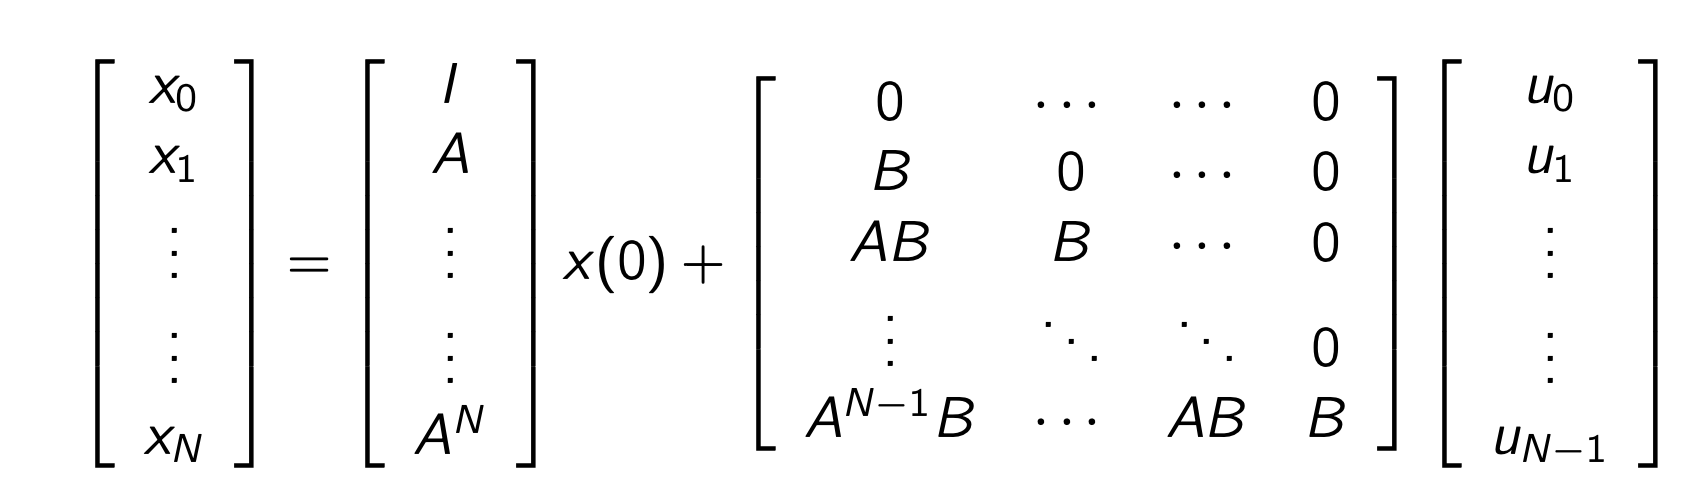
\includegraphics[width=0.6\linewidth]{images/batch.png}
\end{center}

Or in compact notation as $X = S^x x(0) + S^uU$ and with $\Bar{Q} = \text{blockdiag}(Q, \cdots, Q, P)$ , $\Bar{R} = \text{blockdiag}(R, \cdots, R)$. 
The cost function becomes:
\begin{align*}
J(x(0), U)  &= X^T\Bar{Q}X + U^T\Bar{R}U \\
&= U^THU + 2x(0)^TFU + x(0)^TS^{xT}\Bar{Q}S^xx(0)
\end{align*}
with $ H = (S^u)^T\Bar{Q}S^u + \bar{R}$ and $F = (S^x)^T\Bar{Q}S^u$. Note that $H \succ 0$. Minimizing $\nabla_U J(x(0), U) = 0$:

\begin{tcolorbox}[eqbox]
\begin{align*}
U^\star &= -H^{-1}F^Tx(0) \\
J^\star &= -x(0)^TFH^{-1}F^Tx(0) + x(0)^T(S^x)^T\Bar{Q}S^xx(0)
\end{align*}
\end{tcolorbox}

\subsubsection{Recursive approach}
From (\ref{LQR}) we start solving for time $N-1$, obtaining the recursive formula:

\begin{tcolorbox}[eqbox]
\begin{align*}
u_i^\star &= -(B^TP_{i+1}B + R)^{-1}B^TP_{i+1}Ax(i) = F_{i}x_{i} \\
P_i &= A^TP_{i+1}A + Q \\
    &\quad - A^TP_{i+1}B(B^TP_{i+1}B + R)^{-1}B^TP_{i+1}A \\
J^\star_{i}(x(i)) &= x(i)^TP_ix(i)
\end{align*}
\end{tcolorbox}
\textbf{Batch} vs \textbf{Recursive}: batch adapts more easily to constraints; recursive is more efficient and robust to uncertainties.

\textbf{ARE} ($N\to\infty$): steady-state $P_\infty$, $F_\infty = -(B^TP_\infty B+R)^{-1}B^TP_\infty A$
\begin{itemize}[leftmargin=*]
    \item $u^\star(k) = F_\infty x(k)$ $\Rightarrow$ closed loop \textbf{asymptotically stable}
    \item $J^\star = x^TP_\infty x$ is a \textbf{Lyapunov function} of $x(k+1)=(A+BF_\infty)x(k)$
\end{itemize}

\subsection{Convex Optimization}
The standard form is:
\begin{equation} \label{eq:opt_standard_form}
\begin{aligned}
\min_{x \in \text{dom}(f)} \quad & f(x) \\
\text{subj. to} \quad & g_i(x) \leq 0 \\
& h_i(x) = 0 
\end{aligned}
\end{equation}
The $i^{th}$ inequality constraint $g_i(x) \leq 0$ is active at $\Bar{x}$ if $g_i(\Bar{x}) = 0$, otherwise it is inactive. Equality constraints are always active. 
\subsubsection{Convex Sets}
A set is a \textbf{convex set} if and only if for $x$ and $y$ $\in \mathcal{X}$:
\begin{center}
    $\lambda x + (1-\lambda)y \in \mathcal{X}, \forall \lambda \in [0,1], \forall x, y \in \mathcal{X}$
\end{center}

\begin{enumerate}
    \item \textbf{Hyperplane}: Defined as $a^Tx = b$ (\textit{affine}).
    \item \textbf{Halfspace}: $a^Tx \leq b$ Everything on one side of the Hyperplane.
    \item \textbf{Polyhedron}:  $Ax \leq b$ Intersection of a finite number of closed halfspaces.
    \item \textbf{Polytope}: A bounded polyhedron.
    \item \textbf{Ellipsoid}: $(x-x_c)^TA^{-1}(x-x_c) \leq 1$ with $x_c$ the center and $A \succ 0$.
    \item \textbf{Norm Balls}: $ \| x - x_c \|_p \leq r$ with a radius $r$ and a norm $p$
\end{enumerate}
\textbf{The intersection of two or more convex sets is itself convex.} (Union not convex in general)

\subsubsection{Convex Functions}
A function is convex iff dom(f) is convex and $f(\lambda x + (1-\lambda)y) \leq \lambda f(x) + (1-\lambda)f(y)$.
\begin{enumerate}
    \item \textbf{First-order condition}: convex iff $f(y) \geq f(x) + \nabla f(x)^T(y-x)$
    \item \textbf{Second-order condition}: convex iff $\nabla^2f(x) \succeq 0$
\end{enumerate}
\begin{itemize}
    \item \textbf{Affine}: $ax + b$ for any $a,b \in \mathbb{R}$
    \item \textbf{Exponential}: $e^{ax}$ for any $a \in \mathbb{R}$
    \item \textbf{Powers}: $x^\alpha$ on $\mathbb{R}_{++} \text{ and } \alpha \geq 1 \text{ or } \alpha \leq 0$
    \item \textbf{Vector norms}: $\|x\|_p$ for $p \geq 1$
\end{itemize}

\textbf{Operations that preserve convexity}: Non-negative weighted sum, Composition with affine function, Pointwise maximum or supremum, Partial minimization,...

\subsubsection{Optimality Conditions}
For a convex problem of the form (\ref{eq:opt_standard_form}), the \textbf{Lagrangian Function} is defined as $L(x, \lambda, \nu) = f(x) + \sum_{i =1}^m \lambda_i g_i(x) + \sum_{i =1}^p \nu_i h_i(x)$ The \textbf{dual function} is defined as $d(\lambda,\nu) = \inf_x L$, it is  \textbf{always concave} and generates a \textbf{lower bound} $d(\lambda, \nu) \leq p^\star$. The dual problem $ d^\star = \max d(\lambda, \nu)$ subject to $\lambda \geq 0$ is \textbf{always convex} even if the primal is not.\vspace{4pt}

If there is at least one strictly feasible point (for convex problems), then $p^\star = d^\star$ (\textbf{Slater Condition}). Moreover the \textbf{KKT conditions} are defined as
\begin{enumerate}
    \item \textbf{Stationarity}: $\nabla_x L = \nabla f(x^\star)+ \sum \lambda_i^\star \nabla g_i(x^\star) + \sum\nu_i^\star \nabla h_i(x^\star) = 0$
    \item \textbf{Primal Feasibility}: $h_i(x^\star) = 0$ and $g_i(x^\star) \leq 0$
    \item \textbf{Dual Feasibility}: $\lambda^\star \geq 0$
    \item \textbf{Complementarity Slackness}: $\lambda^\star_i g_i(x^\star)= 0$
\end{enumerate}
For Convex with Slatter condition they are \textbf{necessary and sufficient}, but in general just \textbf{necessary}.

\subsubsection{Sensitivity Analysis}

\[
\begin{array}{@{}c@{\qquad}|@{\qquad}c@{}}
    \begin{aligned}
        \min_{x} \quad & f(x) \\
        \text{subj. to} \quad & g_i(x) \le u_i \quad i=1\ldots m \\
        & h_i(x) = v_i \quad i=1\ldots p,
    \end{aligned}
    &
    \begin{aligned}
        \max_{\nu, \lambda} \quad & d(\nu, \lambda) - u^\top \lambda - v^\top \nu \\
        \text{subj. to} \quad & \lambda \ge 0
    \end{aligned}
\end{array}
\]

Assuming strong duality for the original unperturbed problem, weak duality for the perturbed case implies:
\[
    p^\star(u,v) \ge d^\star(\nu^\star, \lambda^\star) - u^\top\lambda^\star - v^\top\nu^\star = p^\star(0,0) - u^\top\lambda^\star - v^\top\nu^\star
\]

\begin{itemize}
    \item \textbf{Global Sensitivity:} Evaluated by varying $\lambda_i^\star, \nu_i^\star$ and $u_i, v_i$.
    
    \item \textbf{Local Sensitivity:} If $p^\star(u, v)$ is differentiable at $(0, 0)$, then:
    \[
        \lambda_i^\star = -\frac{\partial p^\star(0, 0)}{\partial u_i}, \qquad \nu_i^\star = -\frac{\partial p^\star(0, 0)}{\partial v_i}
    \]
    \begin{itemize}
        \item $\lambda_i^\star$ is the sensitivity of $p^\star$ relative to the $i^{\text{th}}$ inequality.
        \item $\nu_i^\star$ is the sensitivity of $p^\star$ relative to the $i^{\text{th}}$ equality.
    \end{itemize}
\end{itemize}

\vspace{2.5em}
\begingroup
\raggedright

\section{Nominal MPC}
\subsection{Constrained Finite Time Optimal Control (CFTOC)}
Solving \ref{eq:opt_standard_form} for an infinite horizon is \textbf{untractable}, that's why we solve it for a finite horizon N. $J^\star(x(k)) = \min_u I_f(x_N) + \sum^{N-1}_{i=0}I(x_i, u_i)$, where $I_f = x_N^{T}Px_N$ approximates the tail of the cost and $I = x_i^TQx_i + u_i^TRu_i$. This can be turned into a QP Problem of the form:

\begin{equation}
\begin{aligned}
\min_{z \in \mathbb{R}^n} \quad & \frac{1}{2}z^THz + q^Tz + r \\
\text{subj. to} \quad & Gz \leq h \\
& Az = b 
\end{aligned}
\end{equation}
\subsubsection{Without Substitution}
\begin{center}
\setlength{\tabcolsep}{1pt}
\renewcommand{\arraystretch}{0}
\begin{tabular}{cc}
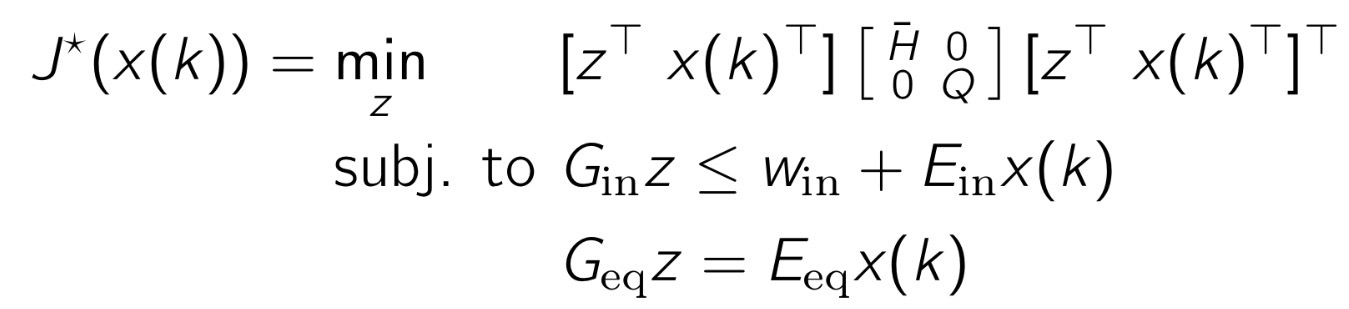
\includegraphics[width=0.49\linewidth]{images/CFTOC/without/problem.jpg} &
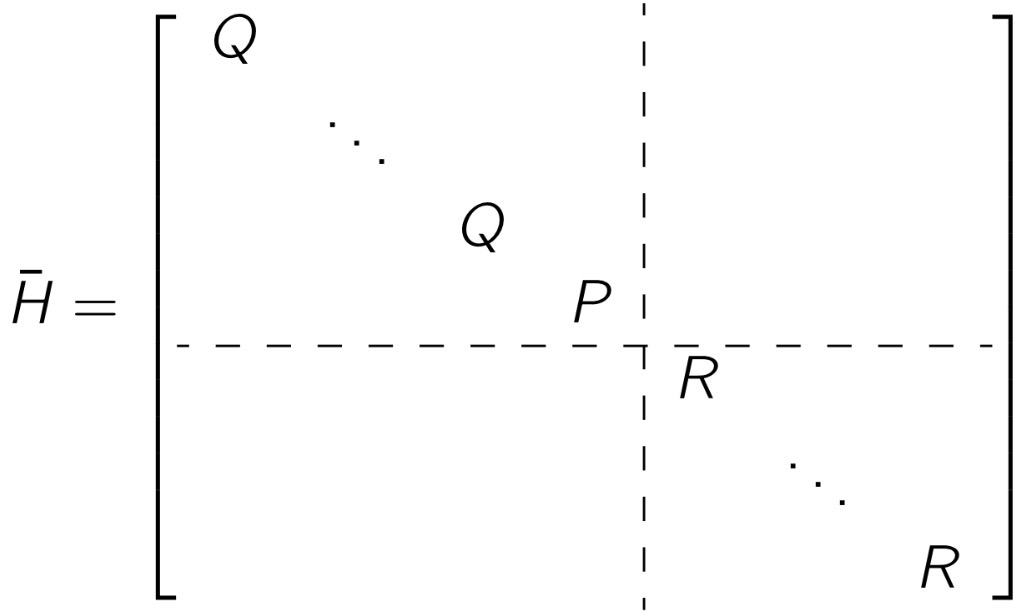
\includegraphics[width=0.29\linewidth]{images/CFTOC/without/H.jpg} \\
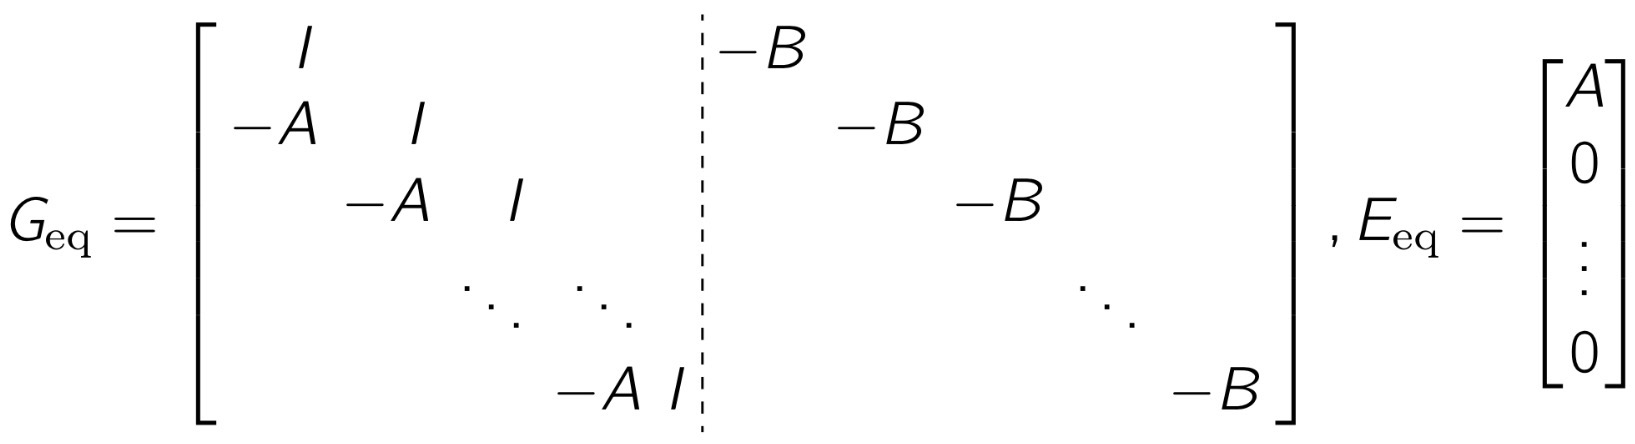
\includegraphics[width=0.49\linewidth]{images/CFTOC/without/equality.jpg} &
\includegraphics[width=0.39\linewidth]{images/CFTOC/without/inequality.jpg}\\
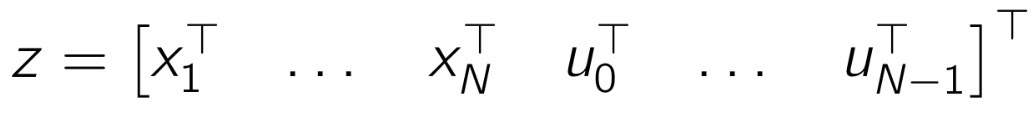
\includegraphics[width=0.29\linewidth]{images/CFTOC/without/z.jpg} &
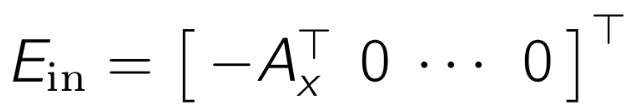
\includegraphics[width=0.19\linewidth]{images/CFTOC/without/E_in.jpg}
\end{tabular}
\end{center}
\vspace{-0.5em}
\subsubsection{With Substitution}
Idea: Substitute the state equations $x_{i+1}=Ax_i+Bu_i\;\;x_0=x(k)$
\begin{itemize}
    \item \textbf{Step 1}: Rewrite the cost as: \\
    $J(x(k),U)=U^THU+2\,x(k)^TFU+x(k)^TYx(k)$\\
    $J=\begin{bmatrix}U^T & x(k)^T\end{bmatrix} \begin{bmatrix}H & F^T \\F & Y\end{bmatrix}\begin{bmatrix}U^T& x(k)^T\end{bmatrix}^T$
    \item \textbf{Step 2}: Rewrite the constraints compactly: \\
    $GU\leq w\,+\,Ex(k)$\\
    Feasible sets: $\mathcal{X}=\{ x\,|A_xx\leq b_x\}$, $\mathcal{U}=\{ u\,|A_uu\leq b_u\}$, $\mathcal{X}_f=\{ x\,|A_fx\leq b_f\}$\\
    Reformulation:
    \begin{enumerate}
        \item $A_xx\leq b_x \rightarrow\;A_xS^UU\leq b_x-A_xS^xx(k)$
        \item $A_uU\leq b_u$
        \item $\boldsymbol{0}\leq b_x-A_xx(k)$\\
        $\rightarrow$ Build resulting $G,\, E\,$ and $w$.
    \end{enumerate}
\end{itemize}
\subsubsection{Comparisons}
$\forall\, \boldsymbol{x}\in \mathbb{R}^n,\,\boldsymbol{u}\in\mathbb{R}^m, horizon \rightarrow N$ 
{\small
\begin{tabularx}{\linewidth}{l|X|X}
 & WITH substitution & WITHOUT substitution \\
\hline
\# variables 
& $Nm$, $z=U$ 
& \makecell[l]{$N(m+n)$ \; $z=\begin{bmatrix}X & U\end{bmatrix}^T$} \\

Pros \& Cons 
& \makecell[l]{less variables \\ evtl. badly conditioned \\ extra computation}
& \makecell[l]{more variables \\ sparse} \\
\end{tabularx}
}


\subsubsection{$\infty$ and $1$ Norm Transformations (Reformulation in \textbf{epigraph} form)}
\noindent
\begin{minipage}[t]{0.48\linewidth}
\small
\begin{align*}
&\min_{x} \|x\|_\infty \text{ s.t. } Fx \leq g \\
&\Rightarrow \min_{x,t} t \text{ s.t. } Fx \leq g,\ -\mathbf{1}t \leq x \leq \mathbf{1}t
\end{align*}
\end{minipage}%
\hfill
\begin{minipage}[t]{0.48\linewidth}
\small
\begin{align*}
&\min_{x} \|x\|_1 \text{ s.t. } Fx \leq g \\
&\Rightarrow \min_{x,t} \mathbf{1}^T t \text{ s.t. } Fx \leq g,\ -t \leq x \leq t
\end{align*}
\end{minipage}


\subsection{Invariance}
\textbf{Constr. Control}:$\;x(k+1)=g(x(k),u(k))\;\forall x,u\in \mathcal{X},\mathcal{U}$\\
\textbf{Goal}: Find control law $u(k)=\kappa(x(k))$ s.t.
\begin{enumerate}
    \item $\{x(k)\}\subset\mathcal{X},\;\{u(k)\}\subset\mathcal{U}\;\;\forall k \rightarrow\textbf{Invariance}$
    \item Stability: $\lim_{k\rightarrow\infty}x(k)=0$
    \item Performance optimization
    \item Maximization of set: $\{x(0)|\;\;1-3\; satisfied\}$
\end{enumerate}
\textbf{Definitions}
\begin{enumerate}
    \item \textbf{Invariance}: Region s.t. the \textbf{autonomous system} (e.g. $x(k+1)=g(x(k))$) satisfies the constraints $\forall t$
    \item \textbf{Control Invariance}: Region in which there \textbf{exists a controller $\kappa$} (e.g. $x(k+1)=g(x(k),\kappa(x(k)))$) s.t. constraints are satisfied $\forall t$
\end{enumerate}


\textbf{Positively Invariant Set}\\ $\mathcal{O}$ is positively invariant for the \textbf{autonomous} system if $x(k)\in \mathcal{O} \Rightarrow x(k+1)\in \mathcal{O},\;\forall k\in\{0,1,...\}$\\
\textbf{Maximal Positively Invariant Set $\mathcal{O}_{\infty}$}\\
The set $\mathcal{O}_\infty\subset\mathcal{X}$ is a maximal positively invariant set w.r.t. $\mathcal{X}$ if:\\ 1) $\mathcal{O}_\infty$ is positively invariant and 2) it contains all positive invariant sets\\
\textbf{Pre Set} Given a set $S$ and the dynamics $x(k+1)=g(x(k))$, the pre set of S is: $pre(S):=\{x|\,g(x)\in S\}$\\
\textbf{e.g. Pre-set computation for linear autonomous systems}\\
Given set $S$ and dynamics $x(k+1)=Ax(k)$, then $pre(S):=\{x|\;Ax\in S\}$.\\
Assuming $S:=\{x|\;Fx\leq f\}\rightarrow pre(S)=\{x|\;FAx\leq f\}$\\
\textbf{Geometric condition for invariance}\\
Set $\mathcal{O}$ is positively invariant iff: $\mathcal{O}\subseteq pre(\mathcal{O}) \Leftrightarrow pre(\mathcal{O})\cap\mathcal{O}=\mathcal{O}$\\

\subsubsection{Algorithm to compute the maximal positively invariant set} $\mathcal{O}_\infty$ for $x(k+1)=g(x(k))$ \, \textbf{Input:} $g, \mathcal{X}$\, \textbf{Output:} $\mathcal{O}_\infty$\\
1. $\Omega_0 \leftarrow \mathcal{X}$\\
2. $\Omega_{i+1} \leftarrow \text{pre}(\Omega_i) \cap \Omega_i$\\
\hspace*{1em} \textbf{if} $\Omega_{i+1} = \Omega_i$ \textbf{then} \textbf{return} $\mathcal{O}_\infty = \Omega_i$ \textbf{else} repeat step 2.

\subsubsection{Control Invariance}
$\mathcal{C}\subseteq\mathcal{X}$ is control invariant if: $x(k)\in\mathcal{C}\Rightarrow\exists\;u(k)\in\mathcal{U}\; \text{s.t.}\;g(x(k),u(k))\in\mathcal{C}\;\;\forall k\in \mathbb{N}^+$\\
\textbf{Maximal Control Invariant Set $\mathcal{C_\infty}$}: $\mathcal{C}_\infty$ is maximal control invariant for $x(k+1)=g(x(k),u(k))$ if $\rightarrow$ 1) Control invariant and 2) contains all control invariant sets\\
\textbf{Calculation of Control invariant sets}:\\
Pre set $\rightarrow pre(S):=\{x|\;\exists u\in \mathcal{U}\ \text{s.t}\;g(x,u)\in S\}$\\

A set $\mathcal{C}$ is control invariant iff $\mathcal{C}\subseteq pre(\mathcal{C})$. Same algorithm as above
can be used.\\

\subsubsection{Pre Set Computation: Controlled system}
Given $x(k+1)=Ax(k)+Bu(k)$ with constraints $u(k)\in \mathcal{U}:=\{u|\;Gu\leq g\}$ and the set $S:=\{x| Fx\leq f\}$.\\
Then:
\begin{align*}
pre(S) &= \{x\,|\;\exists u\in\mathcal{U},\; Ax+Bu\in S\}\\
&= \{x\,|\;\exists u\in\mathcal{U},\; FAx+FBu\leq f\}\\
&= \left\{ x \;\middle|\; \exists u,\;
\begin{bmatrix}FA & FB \\ 0 & G\end{bmatrix}
\begin{bmatrix}x \\ u \end{bmatrix}
\leq
\begin{bmatrix}f \\ g\end{bmatrix}
\right\}
\end{align*}
$\rightarrow$ \textbf{projection operation}\\
\textbf{From Control invariant set $\rightarrow$ Control law}:
Synthesizing a control law $\kappa(x)$ from a control invariant set through optimization problem below:\\
$\kappa(x):=\text{argmin}_u\{f(x,u)|\;g(x,u)\in\mathcal{C},u\in\mathcal{U}\}$\\
NB: 1)$f(x,u)$ is any function, 2) system satisfies constraints but doesn't necessarily converge.\\
Control invariant set is a \textbf{powerful object}, and \textbf{if computable} it provides a direct method for determining a control law satisfying the constraints.\\
\textbf{Issue}: They are \textbf{not always computable} $\rightarrow$ MPC implicitly describes a control invariant set well representable and computable.

\subsection{Practical Computation of invariant sets}

\subsubsection{Polytopes}
  \textbf{Convex hull}: for any subset $S\in\mathbb{R}^d$, co($S$) of S $\rightarrow$ intersection of all convex sets containing S (\textit{smallest convex set containing $S$})\\
  \textbf{Proposition: Convex hull}: convex hull of a set of points $\{v_1,...,v_k\}\in\mathbb{R}^d\rightarrow \text{co($\{v_1,...,v_k\}$}):=\{x|\;x=\sum_i\lambda_iv_i\;,\;\lambda_i\geq0\;,\;\sum_i\lambda_i=1\;\forall i=1,...,k\}$\\
  \textbf{Minkowski-Weyl Theorem}: For $P\subseteq\mathbb{R}^d$ the statements below are equivalent:\\
  \begin{enumerate}
      \item $P$ is a polytope (i.e. $\exists\; A\in\mathbb{R}^{m\,\text{x}\,d},\;b\in\mathbb{R}^m \;\text{s.t.}\;P=\{x|\;Ax\leq b\}$)
      \item $P$ is finitely generated (i.e. $\exists\;\{v_i\}\;\text{s.t.}\; P=\text{co}(\{v_1,...,v_s\})$)
  \end{enumerate}
  \textbf{Examples: Polytopes in MPC}\\
  \begin{itemize}
  \item\textbf{Rate constraints}:\\$||x(k)-x(k+1)||_\infty\leq \alpha\;\Rightarrow\;\begin{bmatrix}I & -I \\ -I & I\end{bmatrix}\begin{bmatrix}x(k) \\ x(k+1)\end{bmatrix}\leq \boldsymbol{1}\alpha$\\
  $\rightarrow$ Polytopes in MPC commonly desribed by \textbf{inequalities}
  \end{itemize}
\textbf{Intersection of Polytopes}: \\Intersection $I\subseteq\mathbb{R}^n$ of sets $S\subseteq\mathbb{R}^n, \;T\subseteq\mathbb{R}^n\;\rightarrow\;I=S\cap T:=\{x|\;x\in S \;\text{and}\; x\in T\}$\\
\textbf{Subset Test}: Is $P:=\{x|\;Cx\leq c\}$ contained in $Q:=\{x|\;Dx\leq d\}$ ?\\ $\rightarrow$ \textbf{True} if $P\subset\{x|\;D_ix\leq d_i\}$ for each row $D_i$ of $D$\\
$\rightarrow$ \textbf{support function} of the set P: $h_P(D_i):=\text{max}_x\,D_ix\;\;\text{subj. to}\;Cx\leq c$ ($h_P(D_i)\leq d_i\;\forall i$)\\

\subsubsection{Ellipsoids}
\textbf{Ellipse}: $E:=\{x|\;(x-x_c)^TP(x-x_c)\leq1\}$ with P$\succeq0$ sym. in $\mathbb{R}^{n\,\text{x}\,n}$ and $x_c\in \mathbb{R}^n$
\textbf{Lemma: Invariant set from Lyapunov function}: $V:\mathbb{R}^n\rightarrow\mathbb{R}$ is a Lyapunov fct. for the system $x(k+1)=g(x(k))$, then $Y:=\{x|\;V(x)\leq \alpha\}$ is \textbf{invariant} $\forall\;\alpha\geq0$\\
\textbf{Goal}: find largest $\alpha$ s.t.:$Y_\alpha:=\{x|\;x^TPx\leq \alpha\}\subset\mathcal{X}:=\{x|\;Fx\leq f\}$\\

\textbf{Maximum ellipsoidal invariant set}: largest ellipsoid contained in a polytope, with
\[
\alpha^\star=\max_\alpha\{\alpha\mid \|P^{-1/2}F_i^\top\|^2\alpha\le f_i^2,\ \forall i\}=\min_i\frac{f_i^2}{F_iP^{-1}F_i^\top}.
\]


\subsection{Feasibility and Stability}
\textbf{Potential issues} with MPC:
\begin{enumerate}
    \item \textbf{No feasibility guarantee} \rightarrow MPC evtl. has no solution
    \item \textbf{No stability guarantee} \rightarrow Trajectories evtl. do not converge to origin
\end{enumerate}

\begin{center}
\scriptsize
\setlength{\tabcolsep}{5pt}
\renewcommand{\arraystretch}{1.15}
\begin{tabular}{|
>{\centering\arraybackslash}m{0.14\linewidth}|
>{\centering\arraybackslash}m{0.35\linewidth}|
>{\centering\arraybackslash}m{0.41\linewidth}|}
\hline
\textbf{Horizon} & \textbf{Feasibility} & \textbf{Stability / Cost} \\ \hline
$N\to\infty$
& Closed-loop trajectory always feasible
& As in LQR: open loop = closed loop; finite cost
  $\Rightarrow x_k,u_k\to0$ \\ \hline
Finite $N$
& Finite-horizon OCP may become infeasible
& Inputs may not drive the system to the origin \\ \hline
\end{tabular}
\end{center}

Issues caused by use of \rightarrow \textbf{short sighted strategies}\\
\textbf{Goal}: Design finite horizon \rightarrow approximate infinite horizon\\
\textbf{Idea}: Introduce terminal cost and constraints to ensure feasibility and stability (\textcolor{red}{mimic infinite horizon})
$J^*(x(k))= \text{min}_U \;\textcolor{red}{l_f(x_N)}\;+\;\sum_{i=0}^{\textcolor{red}{N}-1}l(x_i,u_i)$, $\textcolor{red}{x_N}\in\textcolor{red}{\mathcal{X}_f}$\\

\textbf{Recursive feasibility}: showing the existence of a feasible control sequence at all times when starting from a feasible initial point\\
\textbf{Stability}: showing that the optimal cost function is a Lyapunov function, were \textbf{proven in lecture}:\\ 
for cases: 1) Terminal constraint: $x_N=0$, 2) Terminal constraint in some convex set $x_N\in\mathcal{X}_N$\\


\subsubsection{Lyapunov Stability}
\begin{itemize}
    \item Asymptotic stability: Eqb. point $\bar{x}\in\Omega$ is asy. stable in the set $\Omega\in\mathbb{R}^n$ if it is Lyap. stable and \textbf{attractive}, i.e.
    $\text{lim}_{k\rightarrow\infty}\;||x(k)-\bar{x}||=0\,,\;\forall x(0)\in\Omega$\\
    \textbf{Global asy. stability} if asy. stable and $\Omega=\mathbb{R}^n$
    \item Lyapunov fct.: Fct. $V:\mathbb{R}^n\rightarrow\mathbb{R}$ s.t.$V(0)=0\; \text{and}\;V(x)>0\; \forall x\in\Omega\backslash\{0\}$\\
    $V(g(x))-V(x)\leq-\alpha(x)\;\forall x\in\Omega\backslash\{0\}$, $\alpha(x):\mathbb{R}^n\rightarrow\mathbb{R}$
    \item Lyapunov (asy.) stability: For systems admitting Lyap. fcts. $V(x)$, $x=0$ is \textbf{asymptotically stable} in $\Omega$
\end{itemize}
\subsubsection{Feasibility and stability guarantees proof for $\mathcal{X}_\text{f}=0$}
\begin{enumerate}
\item Goal: Prove recursive feasibility
\begin{itemize}
    \item Assume feasibility of $x(k)$ and $\{u_0^*\,,\,u_1^*\,,\,...\,,\,u_{N-1}^*\}$ optimal control sequence at $x(k)$ with $\{x(k)\,,\,x_1^*\,,\,...\,,\,x_{N}^*\}$ corresponding state trajectory
    \item Apply $u(k)=u_0^*$ and let the system evolve to $x(k+1)=A\,x(k)+B\,u(k)=x_1^*$
    \item At $x(k+1)$ the control sequence $\tilde{U}=\{u_1^*\,,\,u_2^*\,,...\,,u_{N-1}^*\,,\textcolor{red}{0}\}$ is \textbf{feasible}.\\
    $A\,x_N^*+B\cdot0=0$ \Rightarrow Feasible set is invariant, terminal constraint is satisfied, Feasible set is invariant \rightarrow \textcolor{red}{Recursive feasibility}
\end{itemize}
\item Goal: Show $J^*(x(k+1))<J^*(x(k))\;\forall x(k)\neq0$\\
$\tilde{U}=\{u_1^*\,,\,u_2^*\,,...\,,u_{N-1}^*\,,\textcolor{red}{0}\}$, $\tilde{X}=\{x_1^*\,,\,...\,,\,x_{N}^*\,,\,\textcolor{red}{0}\}$\\
$J^*(x(k))=l_f(x_N^*)+\sum_{i=0}^{N-1}l(x_i^*\,,\,u_i^*)\,,\text{with }l_f(x_N^*)=0$\\
$J^*(x(k+1))\leq\tilde{J}(x(k+1))=\sum_{i=1}^{N-1}l(x_i^*\,,\,u_i^*)+l(x_N^*\,,\,0)$\\
$=\sum_{i=0}^{N-1}l(x_i^*\,,\,u_i^*)-l(x_0^*\,,\,u_0^*)+l(x_N^*\,,\,0)$\\
$=J^*(x(k))-l(x(k)\,,\,u_0^*)+l(0\,,\,0)\;\text{where }l(0\,,\,0)=0$\\
\Rightarrow $J^*(x)$ is a \textcolor{red}{Lyapunov function} \rightarrow \textcolor{red}{Asymptotic Lyapunov stability}
\end{enumerate}
\textbf{Extension to more general terminal sets}\\
\textbf{Problem:} The constraint $x_N=0$ reduces the size of the feasible set\\
\textbf{Goal:} Make use of $\mathcal{X}_f$ to increase the region of attraction \\\rightarrow Generalize proof to the constraint $x_N\in\mathcal{X}_\text{f}$\\

\textbf{Def: Invariant set}\\
$\mathcal{O}\rightarrow \textbf{positively invariant}$ for $x(k+1)=g_{cl}(x(k))$ if:\\
$x(0)\in\mathcal{O}\Rightarrow x(k)\in\mathcal{O}, \;\forall k\in\mathbb{N}_+$\\
\subsubsection{Stability of MPC - Main results}
Assumptions (\textbf{sufficient} conditions that guarantee stability and feasibility of the MPC)
\begin{enumerate}
    \item \textbf{Positive definite stage cost} (strictly pos. and only zero at the origin)
    \item \textbf{Recursive Feasibility}: Terminal set is \textbf{invariant} under the local control law $\kappa_\text{f}(x_i)$:\\
    $x_{i+1}=A\,x_i+B\kappa_\text{f}(x_i)\in\mathcal{X}_\text{f},\;\forall x_i\in\mathcal{X}_\text{f}$\\
    All state and input constraints are satisfied:\\
    $\mathcal{X}_\text{f}\subseteq\mathcal{X}\,,\,\kappa_\text{f}(x_i)\subseteq\mathcal{U},\;\forall x_i\in\mathcal{X}_\text{f}$
    \item \textbf{Stability}: Terminal cost is a continuous \textbf{Lyapunov function} in the terminal set $\mathcal{X}_\text{f}$ and:\\
    $l_\text{f}(x_{i+1})-l_\text{f}(x_i)\leq-l(x_i\,,\,\kappa_\text{f}(x_i))$
\end{enumerate}
Plan for N steps \rightarrow use local controller that keeps the system in a stable manner in the terminal set (condition 3 ensures stability)\\
\textbf{Theorem (Closed-Loop System Stability)}:\\
Under those 3 assumptions, the closed-loop system under the MPC control law $u_0^*(x)$ is asymptotically stable and the set $\mathcal{X}_\text{N}$ (Region of Attraction) is positively invariant for the system\\
$x(k+1)=A\,x(k)+B\,u_0^*(k)$\\
\textbf{Stability of MPC - Outline of the Proof}\\
\begin{itemize}
    \item Assume feasibility of $x(k)$ and $\{u_0^*\,,\,...\,,\,u_{N-1}^*\}$ the optimal control sequence computed at $x(k)$ with $\{x(k)\,,\,x_1^*\,,\,...\,,\,x_N^*\}$ the resulting state trajectory
    \item At $x(k+1)=x_1^*$ the sequence: $\tilde{U}=\{u_1^*\,,\,...\,,\,\kappa_\text{f}(x_N^*)\}$ is \textbf{feasible} ($x_N^*\in\mathcal{X}_\text{f}$\rightarrow $\kappa_\text{f}(x_N^*)$ is feasible and $A\,x_N^*+B\,\kappa_\text{f}(x_N^*)\in\mathcal{X}_\text{f}$)\\
    \Rightarrow Terminal constraint provides \textcolor{red}{Recursive feasibility}
\end{itemize}
\textbf{Asymptotic stability of MPC - Outline of the proof}\\
$J^*(x(k))=\sum_{i=0}^{N-1}l(x_i^*\,,\,u_i^*)+l_\text{f}(x_N^*)$\\
At $x(k+1)=x_1^*\,,\,\tilde{U}=\{u_1^*\,,\,...\,,\,\kappa_\text{f}(x_N^*)\}$ is feasible and sub-optimal:\\
$J^*(x(k+1))\leq\sum_{i=1}^{N-1}l(x_i^*\,,\,u_i^*)+l(x_N^*\,,\,\kappa_\text{f}(x_N^*))+l_\text{f}(A\,x_N^*+B\,\kappa_\text{f}(x_N^*))$\\
$=\sum_{i=0}^{N-1}l(x_i^*\,,\,u_i^*)-l(x_0^*\,,\,u_0^*)+l(x_N^*\,,\,\kappa_\text{f}(x_N^*))+l_\text{f}(A\,x_N^*+B\,\kappa_\text{f}(x_N^*))$\\
$=J^*(x(k))-l(x(k)\,,\,u_0^*)+l_\text{f}(A\,x_N^*+B\,\kappa_\text{f}(x_N^*))-l_\text{f}(x_N^*)+l(x_N^*\,,\,\kappa_\text{f}(x_N^*))$\\
$\Rightarrow J^*(x(k+1))-J^*(x(k))\leq-l(x(k)\,,\,u_0^*)$\\
\textcolor{red}{$J^*(x)$ \textbf{ is a Lyapunov function}}\\
\Rightarrow The closed-loop system under the MPC control law is \textcolor{red}{asymptotically stable}\\
\subsubsection{Choice of terminal sets and cost - Linear system dynamics and quadratic cost}
$J^*(x(k))=\min_U\textcolor{red}{x_N^TPx_N}+\sum_{i=0}^{\textcolor{red}{N}-1}x_i^TQx_i+u_i^TRu_i$ (\textcolor{red}{Terminal cost})\\
subj.to  $x_{i+1}=A\,x_i+B\,u_i, \forall i=0\,,\,...\,,\,N-1$\\
$x_i\in\mathcal{X}\,,\,u_i\in\mathcal{U}\,,\,\forall i=0\,,\,...\,,\,N-1$\\
$\textcolor{red}{x_N\in\mathcal{X}_\text{f}}$ (\textcolor{red}{Terminal constraint})\\
$x_0=x(k)$\\
\begin{itemize}
    \item Formulate unconstrained LQR control law:\\
    $F_\infty=-(B^TP_\infty B+R)^{-1}B^TP_\infty A$\\
    $P_\infty \rightarrow $ solution to DARE
    \item Terminal weight $P=P_\infty$
    \item Terminal set $\mathcal{X}_\text{f}$ maximum invariant set for the cl-system $x_{k+1}=(A+BF_\infty)x_k$\\
    $x_{k+1}=(A+BF_\infty)x_k\in\mathcal{X}_\text{f},\;\forall x_k\in \mathcal{X}_\text{f}$\\
    $\mathcal{X}_\text{f}\subseteq\mathcal{X}\,,\, F_\infty x_k\subseteq\mathcal{U}\,\,\forall x_k\in\mathcal{X}_\text{f}$
\end{itemize}
\begin{enumerate}
    \item Stage cost is positive definite
    \item Terminal set is invariant by construction under the local control law $\kappa_\text{f}(x)=F_\infty x$
    \item Terminal cost is continuous Lyapunov function in the terminal set $\mathcal{X}_\text{f}$ and:\\
    $x_{k+1}^TP_\infty x_{k+1}-x_k^TP_\infty x_k=$\\
    $x_k^T(-P_\infty+A^TP_\infty A+F_\infty^TB^TP_\infty A-F_\infty^TRF_\infty)x_k$\\
    $=-x_k^T(Q+F_\infty^TRF_\infty)x_k$
\end{enumerate}
\rightarrow All assumptions of the feasibility and stability theorem are verified\\


\begingroup

\textbf{Example}:
\begin{enumerate}
    \item Compute the optimal LQR controller and cost matrices:
    $F_\infty,\;P_\infty$.
    
    \item Compute the maximal invariant set $\mathcal{X}_{\mathrm f}$
    for the closed-loop system
    $x_{k+1}=(A+BF_\infty)x_k$, subject to
    \[
    \mathcal{X}_{\mathrm{cl}}
    :=
    \left\{
    x \,\middle|\,
    \begin{bmatrix}
        A_x\\
        A_uF_\infty
    \end{bmatrix}x
    \le
    \begin{bmatrix}
        b_x\\
        b_u
    \end{bmatrix}
    \right\}.
    \]
\end{enumerate}

\endgroup
\textbf{Summary}
\begin{itemize}
    \item Terminal constraint \textbf{sufficient} condition for feasibility and stability
    \item Region of attraction (ROA) without terminal constraint evtl. larger than for MPC with terminal constraint
    \item $\mathcal{X}_\text{f}=0$ simplest choice \rightarrow small ROA for small N
    \item Solutions available for linear systems with quadratic cost
    \item Practically: Enlarge horizon $N$, check stability by sampling
    \item Larger horizon $N$\rightarrow ROA reaches maximum control invariant set
\end{itemize}
\textbf{Sidenotes}: 
\begin{itemize}
    \item From example: Decrease in the prediction horizon causes loss of the stability properties
    \item Inclusion of the terminal cost and constraint provides stability
\end{itemize}
\textbf{Extension to nonlinear MPC}\\
Given nonlinear system dynamics $x(k+1)=g(x(k)\,,\,u(k))$\\
\rightarrow Assumptions on terminal set and constraints: NOT relying on linearity
\rightarrow Lyapunov stability used to analyze stability of nonlinear dynamical systems\\
Issue: determining $\mathcal{X}_\text{f}$ and $l_\text{f}$ can be difficult\\
\textbf{Summary}\\
\textbf{Finite-horizon MPC may not be stable}\\
\textbf{Finite-horizon MPC may not satisfy the constraints for all time}\\
\textcolor{red}{\rightarrow} in contrast infinite-horizon provides stability and invariance\\
\textcolor{red}{\rightarrow} Infinite-horizon faked by: forcing final state to be in invariant set for which there is an invariance-inducing controller


\endgroup
\section{Practical MPC}
\subsection{Practical Issues}
\textbf{MPC: Practical issues}
\begin{enumerate}
    \item \textbf{Tracking}
    \begin{itemize}
        \item Classic MPC formulation: \textbf{regulation of system to the origin}
        \item BUT most commonly: tracking of non-zero output set points  
    \end{itemize}
    \item \textbf{Disturbance rejection}\\
    Issue is that a constant disturbance causes an offset from the origin/ desired point of convergence\\
    \rightarrow Goal: remove offset s.t. system converges to desired set point
    \item \textbf{Feasible set}\\
    Constraints restrict  the set of states for which the optimization problem is feasible (MPC controller only defined in the feasible set)\\
    \rightarrow Make feasible set as large as possible
\end{enumerate}
\subsection{MPC for Reference tracking}
Given: $x(k+1)=A\,x(k)+B\,u(k)$ under the constraint sets $\mathcal{X}=\{x|G_xx\leq h_x\}$, $\mathcal{U}=\{u|G_uu\leq h_u\}$\\
\textbf{Goal}: Drive the system to the desired steady state condition $(x_s\,,\,u_s)$ that yields the desired output $z(k)=Hx(k)\rightarrow r \text{ as } k\rightarrow\infty$\\
\textbf{How is the MPC problem modified in order to achieve tracking?}\\
Target condition \rightarrow $x_s=Ax_s+Bu_s$, $z_s=Hx_s=r$ \Leftrightarrow $\begin{bmatrix}
    I-A &-B \\H&0
\end{bmatrix}\begin{bmatrix}
    x_s\\u_s
\end{bmatrix}=\begin{bmatrix}
    0\\r
\end{bmatrix}$\\
\begin{enumerate}
    \item \textbf{Multiple feasible $u_s$}: find "cheapest" steady state\\
    $\min u_s^TR_su_s$
    subj. to $\begin{bmatrix}
    I-A &-B \\H&0
\end{bmatrix}\begin{bmatrix}
    x_s\\u_s
\end{bmatrix}=\begin{bmatrix}
    0\\r
\end{bmatrix}$, $x_s\in\mathcal{X}_\text{f}\,,\,u_s\in\mathcal{U}$
\item General assumption: feasible problem, BUT if \textbf{NO SOLUTION EXISTS} \\\rightarrow Compute reachable set point closest to $r$\\
$\min (Hx_s-r)^TQ_s(Hx_s-r)$\\
subj. to $x_s=Ax_s+Bu_s,\,x_s\in\mathcal{X},\,u_s\in\mathcal{U}$

\end{enumerate}

\begin{tcolorbox}[eqbox]
\begin{align*}
\min_{U}\quad &
\lVert z_N-Hx_N\rVert_{P_z}^2
+\sum_{i=0}^{N-1}
\left(
\lVert z_i-Hx_s\rVert_{Q_z}^2
+\lVert u_i-u_s\rVert_R^2
\right) \\
\text{s.t.}\quad &
\text{model and constraints},\qquad x_0=x(k).
\end{align*}
\end{tcolorbox}


\subsubsection{Delta formulation for tracking}
Set point tracking \rightarrow regulation problem with coordinate transformation
\begin{itemize}
    \item Define deviation variables:\\
    $\Delta x=x-x_s$, $\Delta u=u-u_s$ \Rightarrow $\Delta x_{k+1}=x_{k+1}-x_s$\\
    $=Ax_k+Bu_k-(Ax_s+Bu_s)$
    $=A\Delta x_k+B\Delta u_k$
    \item Constraints for deviation variables:\\
    $G_xx\leq h_x\Rightarrow G_x\Delta x\leq h_x-G_xx_s$\\
    $G_uu\leq h_u \Rightarrow G_u\Delta u\leq h_u-G_uu_s$
\end{itemize}
\textbf{MPC Problem for tracking in Delta formulation}:\\
\noindent
\begin{minipage}[t]{0.62\linewidth}
\begin{itemize}
    \item Initial state $\Delta x(k)=x(k)-x_s$
    \item Apply regulation to new system in Delta formulation:\\
    \mbox{$\min \sum_{i=0}^{N-1}\Delta x_i^TQ\Delta x_i+\Delta u_i^TR\Delta u_i+V_f(\Delta x_N)$} \\
    s.t. $\Delta x_0=\Delta x(k)$
    \\$\Delta x_{i+1}=A\Delta x_i+B\Delta u_i$\\
    $G_x\Delta x_i\leq h_x-G_x x_s$\\
    $G_u\Delta u_i\leq h_u-G_uu_s$\\
    $\Delta x_N\in \mathcal{X}_\text{f}$
    \item Find optimal sequence of $\Delta U^*$, $U^* = \Delta U^* + U_S$
\end{itemize}
\end{minipage}%
\hfill
\begin{minipage}[t]{0.34\linewidth}
\centering
\vspace{2.5em}
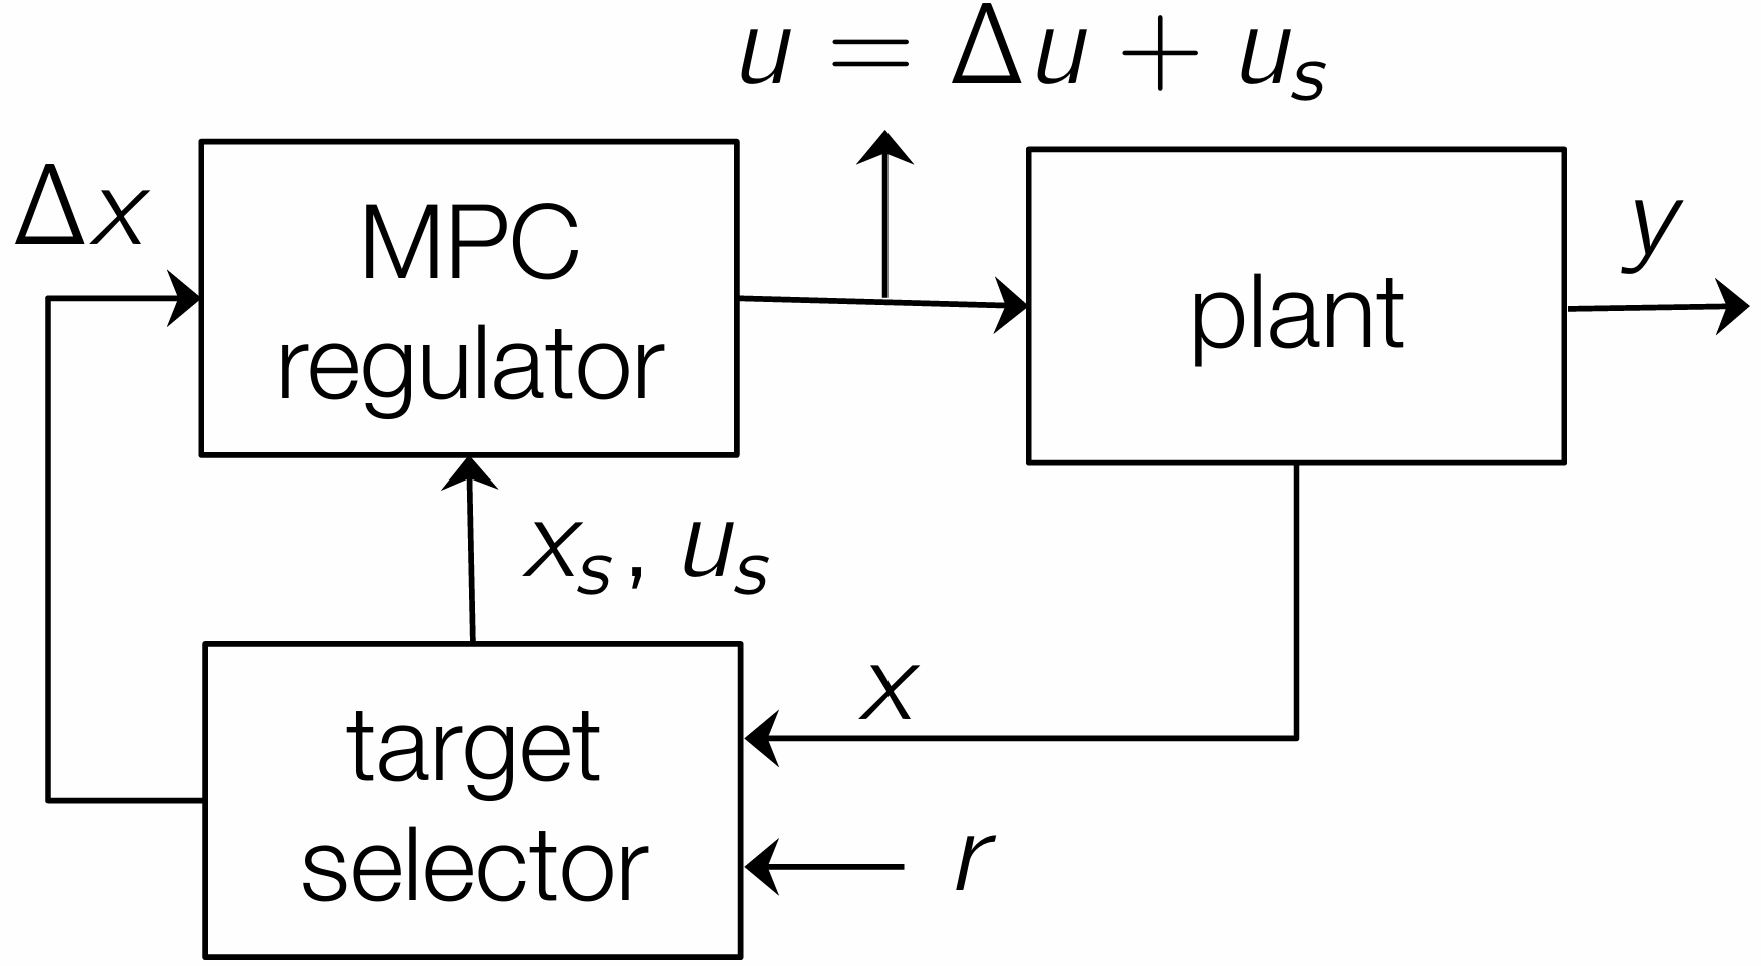
\includegraphics[width=0.9\linewidth]{images/mpc_tracking_diagram.png}
\end{minipage}
\textbf{MPC for tracking: Convergence}\\
Assumption: Feasible target with $x_s\in\mathcal{X}$, $u_s\in\mathcal{U}$ with terminal weight $V_\text{f}$ and constraint $\mathcal{X}_\text{f}$ satisfying:
\begin{itemize}
    \item $(A+BK)x\in\mathcal{X}_\text{f},\;\forall x\in\mathcal{X}_\text{f}$
    \item $V_\text{f}(x(k+1))-V_\text{f}(x(k))\leq-l(x(k)\,,\,Kx(k)),\;\forall x\in\mathcal{X}_\text{f}$
\end{itemize}
IF furthermore the target reference $x_s$, $u_s$ is such that:\\
$x_s\oplus\mathcal{X}_\text{f}\subseteq\mathcal{X}$, $K\Delta x+u_s\in \mathcal{U}$, $\forall \Delta x\in\mathcal{X}_\text{f}$\\
\textcolor{red}{\rightarrow} the cl-system \textcolor{red}{converges to the target reference}\\
$x(k)\rightarrow x_s$, therefore $z(k)=Hx(k)\rightarrow r,\text{ as } k\rightarrow\infty$\\
\textbf{MPC for tracking: Terminal set }\\
Issue: set of feasible targets may be reduced.\\
\rightarrow Enlarge the set of feasible targets by scaling the terminal set for regulation
\begin{itemize}
    \item Scale terminal set by $\alpha$: $\mathcal{X}_\text{f}^{scaled}=\alpha\mathcal{X}_\text{f}$
    \item Thereby invariance is maintained
    \item Choose $\alpha$ s.t. state and input constraints are satisfied (scaling dependent of target)
\end{itemize}
\textbf{Summary: MPC for tracking}\\
\begin{itemize}
    \item Set point tracking problem \Rightarrow Regulation problem after coordinate transformation
    \item If cl-system stable \Rightarrow Set point is achieved
    \item Difficulties:
    \begin{enumerate}
        \item Terminal set is fct. of the target
        \item Ref. change can make the problem infeasible
        \item \textbf{Controller could show offset for unknown model error or disturbances}
    \end{enumerate}
\end{itemize}
\subsubsection{MPC for reference tracking without offset}
\textbf{Constant disturbance acting on the system}:
$x(k+1)=Ax(k)+Bu(k)+B_dd$,\\
$y(k)=Cx(k)+C_dd$\\
\textbf{Goal:} If the system is stabilized in presence of disturbance \\\rightarrow it converges to set point with zero offset\\
Approach in constrained control:
\begin{itemize}
    \item Model the disturbance
    \item Estimate state and disturbance through measurements and models 
    \item Through disturbance estimates find control inputs that remove the offset
\end{itemize}
\textbf{Augmented model}\\
Introduce disturbance model (integral disturbance dynamics)\\
$x_{k+1}=Ax_k+Bu_k+B_dd_k$\\
$d_{k+1}=d_k$\\
$y_k=Cx_k+C_dd_k$\\
Restriction on choice of $B_d,\,C_d$ \rightarrow observability of the augmented model\\
Augmented system is observable iff:
\begin{itemize}
    \item $(A,C)$ is observable
    \item $\begin{bmatrix}
        A-I&B_d\\C&C_d
    \end{bmatrix}$ full column rank ($\text{rank}=n_x+n_d$)\\
    $\rightarrow$ Maximal disturbance dimension $n_d\leq n_y$
\end{itemize}
\textbf{Linear state estimation}\\
State observer for augmented problem\\
$\begin{bmatrix}
    \hat{x}(k+1)\\\hat{d}(k+1)
\end{bmatrix}=\begin{bmatrix}
    A&B_d\\0&I
\end{bmatrix}\begin{bmatrix}
    \hat{x}(k)\\\hat{d}(k)
\end{bmatrix}+\begin{bmatrix}
    B\\0
\end{bmatrix}u(k)+\begin{bmatrix}
    L_x\\L_d
\end{bmatrix}(-y(k)+C\hat{x}(k)+C_d\hat{d}(k))$\\
$\hat{(\cdot)}$\rightarrow estimates of the state and disturbance, $y$ the measured output\\
Error dynamics:\\
$\begin{bmatrix}
    x(k+1)-\hat{x}(k+1)\\
    d(k+1)-\hat{d}(k+1)
\end{bmatrix}=\left(\begin{bmatrix}
    A&B_d\\0&I
\end{bmatrix}+\begin{bmatrix}
    L_x\\L_d
\end{bmatrix}\begin{bmatrix}
    C&C_d
\end{bmatrix}\right)\begin{bmatrix}
    x(k)-\hat{x}(k)\\d(k)-\hat{d}(k)
\end{bmatrix}$\\
\Rightarrow Choose L s.t. error dynamics are asymptotically stable\\


\subsubsection{Offset free tracking}
Lemma: Suppose asymptotically stable observer and $n_y=n_d$\\


\begin{tcolorbox}[eqbox]
\begin{align*}
\text{Observer steady state satisfies: }
\begin{bmatrix}
    A-I&B\\C&0
\end{bmatrix}\begin{bmatrix}
    \hat{x}_\infty\\u_\infty
\end{bmatrix}=\begin{bmatrix}
    -B_d\hat{d}_\infty\\y_\infty-C_d\hat{d}_\infty
\end{bmatrix}
\end{align*}
\end{tcolorbox}

\Rightarrow Observer output tracks measurement $y_\infty$ without offset\\
Goal: Track constant reference $r$: $z(k)=Hy(k)\rightarrow r,\;k\rightarrow\infty$\\
New steady state condition: $\begin{aligned}[t]
    x_s &= Ax_s+Bu_s+B_d\hat{d}_\infty \\
    z_s &= H(Cx_s+C_d\hat{d}_\infty)=r
\end{aligned}$\\
General offset free tracking scheme:
\begin{enumerate}
    \item Estimate state and disturbance $\hat{x},\,\hat{d}$
    \item Obtain $(x_s\,,\,u_s)$ using disturbance estimate
    \item Solve MPC problem using the disturbance estimate $\hat{d}$:\\
    $\min _U\sum_{i=0}^{N-1}(x_i-x_s)^TQ(x_i-x_s)+(u_i-u_s)^TR(u_i-u_s)+V_\text{f}(x_N-x_s)$\\
    subj.to $x_0=\hat{x}(k),\;d_0=\hat{d}(k)$\\
    $x_{i+1}=Ax_i+Bu_i+B_dd_i$\\
    $d_{i+1}=d_i$\\
    $x_i\in\mathcal{X},\,u_i\in\mathcal{U},\,x_N-x_s\in\mathcal{X}_\text{f}$
\end{enumerate}
\begin{minipage}[t]{0.60\linewidth}
\textbf{Summary: offset-free control}\\
Main result: IF
\begin{itemize}
    \item $n_y=n_d$
    \item target steady state problem is feasible
    \item the cl-system converges
\end{itemize}
$\Rightarrow$ Target achieved without offset!
\end{minipage}%
\hfill
\begin{minipage}[t]{0.35\linewidth}
  \centering
  \vspace{-5em}
  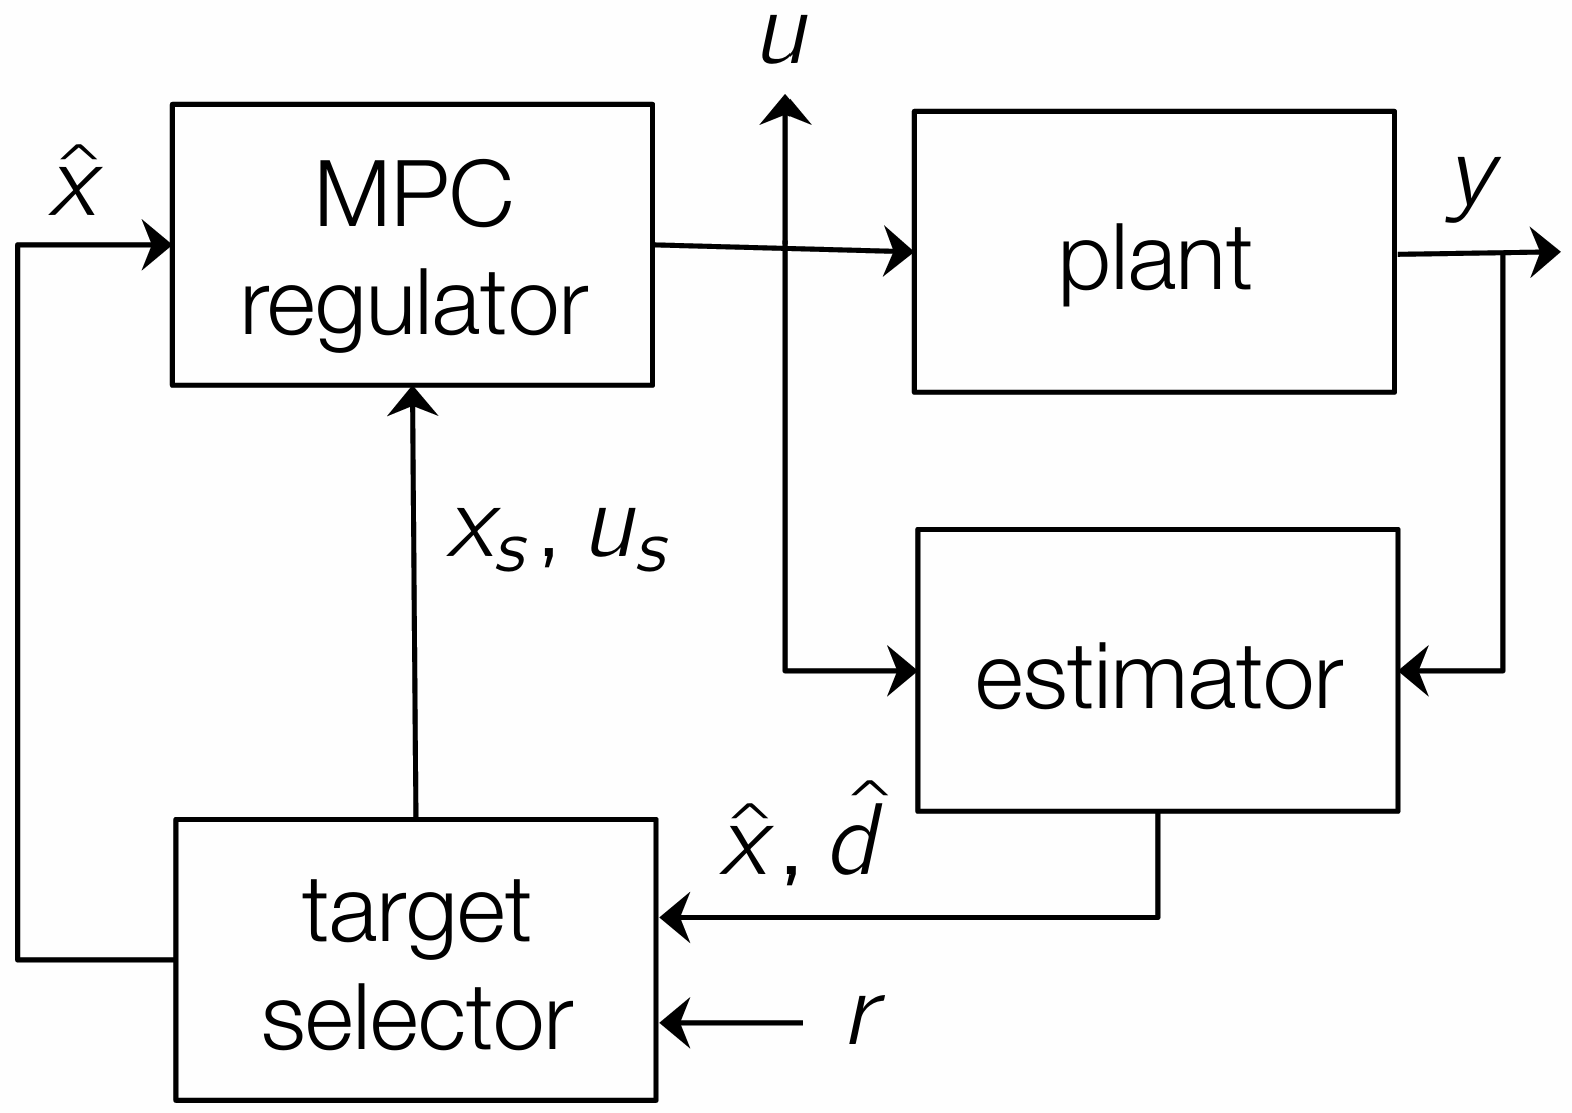
\includegraphics[width=0.9\linewidth]{images/mpc_wo_offset_diagram.png}
\end{minipage}

\subsection{Enlarging the feasible set}
\textbf{Assumptions for Stability of MPC:}\\
\begin{enumerate}
    \item Stage cost is pos. def. (only zero at origin)
    \item Terminal set is \textbf{invariant} under the local control law $\kappa_\text{f}(x_i)$\Rightarrow $x_{i+1}=Ax_i+B\kappa_\text{f}(x_i)\in\mathcal{X}_\text{f},\; \forall x_i\in\mathcal{X}_\text{f}$
    \item Terminal cost continuous Lyapunov function in $\mathcal{X}_\text{f}$ and: $l_\text{f}(x_{i+1})-l_\text{f}(x_i)\leq -l(x_i,\kappa_\text{f}(x_i)),\;\forall x_i\in\mathcal{X}_\text{f}$
\end{enumerate}
\textbf{Important}: Terminal constraint \rightarrow feasible set reduction\\
\textbf{Goal}: MPC without terminal constraint with guaranteed stability\\
\textbf{Note}: Feasible set without terminal constraint is NOT INVARIANT

\subsubsection{MPC without Terminal Set}
    Stability is maintained when removing the terminal constraint if:\\
    1) Initial state in sufficiently small subset of feasible set \;
    2) Horizon $N$ is sufficiently large\\
    \Rightarrow Terminal state satisfies terminal constraint without explicit enforcement in the optimization\\
    \Rightarrow Sol. of finite horizon MPC corresponding to infinite horizon MPC\\
    \textbf{Advantage}: Controller defined in larger feasible set\\
    \textbf{Disadvantage}: Definition of Region of attraction (ROA) or required horizon N difficult \\
    \textbf{Remarks}: Larger horizon length N, ROA \rightarrow maximum control inv. set


    
\subsubsection{Soft constrained MPC}
    Input constraints usually hard vs. State/ output constraints rarely hard\\
    \rightarrow Hard state and output constraints cause complications in the controller implementation
    \Rightarrow In practice: \textbf{State constraints are softened}\\
    \textbf{Objectives}:
\[
\left.
\begin{aligned}
&\text{Minimize violation duration}\\
&\text{Minimize violation size}
\end{aligned}
\right\}
\;\rightarrow\;
\textbf{multi-objective problem}
\]
    \textbf{Soft Constrained MPC problem setup}\\

\begin{tcolorbox}[eqbox]
\begin{align*}
\min_{U,\epsilon}\quad &
\sum_{i=0}^{N-1}\!\left(x_i^\top Qx_i+u_i^\top Ru_i+
\ell_\epsilon(\epsilon_i)\right)
+x_N^\top Px_N+\ell_\epsilon(\epsilon_N)\\[-1mm]
\text{s.t.}\quad &
x_{i+1}=Ax_i+Bu_i,\;
H_xx_i\leq k_x+\epsilon_i,\;
H_uu_i\leq k_u,\;
\epsilon_i\geq0,
\end{align*}
\end{tcolorbox}

    

    \rightarrow State constraints are \textbf{slack variables $\epsilon_i\in\mathbb{R}^p$}\\
    \rightarrow Amount of constraint violation penalized by $l_\epsilon(\epsilon_i)$\\

    \textbf{Original problem}: $\min_zf(z)$\quad
    subj.to $g(z)\leq0$\\
    \textbf{"Softened" problem}: $\min_{z,\epsilon}f(z)+l_\epsilon(\epsilon)$\quad
    subj.to $g(z)\leq \epsilon,\;\epsilon\geq0$\\
    \textbf{Important requirement on $l_\epsilon(\epsilon)$}:
    If original problem has feasible solution $z^*$\\\rightarrow the softened problem should have the same solution $z^*$, and $\epsilon=0$\\
    \textbf{Issue:} E.g. $l_\epsilon(\epsilon)=s\cdot\epsilon^2$ doesn't satisfy this requirement for any $s>0$\\
    \textbf{Main result: Exact Penalty function}\\
    $l_\epsilon(\epsilon)=\nu\cdot\epsilon$ satisfies the requirement for any $\nu>\lambda^*\geq0$ \\($\lambda^*$ is the optimal Lagrange multiplier of teh original problem)\\
    Extension to multiple constraints $g_j(z)\leq0,\,j=1\,,\,...\,,\,r$\\
    $l_\epsilon(\epsilon)=\nu\cdot||\epsilon||_{1/\infty}+\epsilon^TS\epsilon$ ($\nu>||\lambda^*||_D$ and $S\succ0$\rightarrow used to weight violations differently, $||\cdot||_D$: dual of the chosen norm)\\
    \textbf{Properties of the quadratic penalty:}\\
    \rightarrow Increasing $S$ causes \textbf{hardening of the soft constraints} (reduced size of violation BUT longer duration)\\
    \rightarrow $\nu$ large enough: satisfaction of constraints if possible (large $\nu$: increased peak violations and decreasing duration)\rightarrow \textbf{better to keep $\nu$ as small as possible}\\
    \textbf{Summary: Soft constraints}:\\
    \rightarrow Soft constraints recover feasibility when constraints cannot be satisfied\\
    \rightarrow Allow for \textbf{tradeoff btw. violation duration vs. size} \\
    \rightarrow Good closed loop properties  (standard methods of softconstrained MPC: no stability guarantees for unstable ol-systems)\\
    \rightarrow \textbf{Separation of Objectives}: Solve two optimization 1) Min. violation 2) Optimize performance (Simpler to tune but require two optimizations)
\section{Robust MPC}
\vspace{0.5em}
\textbf{Motivation}: MPC relies on a model BUT noise and model inaccuracies can lead to:
\begin{itemize}
    \item Constraint violation
    \item Sub-optimal behavior
    \item Noise prevents the system to converge to a single point\\
\end{itemize}
\textbf{Note}: Possible to incorporate some noise models in the MPC formulation (Hard to solve)\\


\subsection{Uncertainty Models}
\textbf{MPC}: $x(k+1)=g(x(k),u(k))$ \, ; \, \textbf{Reality} $x(k+1)=g(x(k),u(k),w(k);\theta)$ (Noise $\omega(k)$ \& unknown model parameters $\theta$)\\
\textbf{Uncertain constrained system}:\\
$x(k+1)=g(x(k),u(k),w(k);\theta),\;x,u\in\mathcal{X,\mathcal{U}}\quad w\in\mathcal{W}\;\quad \theta\in\Theta$\\
($\mathcal{W},\Theta$) assumed to be compact\\
\textbf{Goal}: Design control law $u(k)=\kappa(x(k))$ s.t.
\begin{enumerate}
    \item Constraint satisfaction: $\{x(k)\}\subset\mathcal{X},\,\{u(k)\}\subset \mathcal{U}$
    \item Stability: Convergence to a neighborhood around the origin
    \item Optimization of expected performance
    \item Maximization of the set $\{x(0)|\text{ Conditions 1-3 satisfied }\}$
\end{enumerate}
\rightarrow This requires assumptions about the random values $w$ and $\theta$

\subsection{Robust invariance}
$\mathcal{O^W}$ is robust positive invariant for the autonomous system $x(k+1)=g(x(k),w(k))$ if:\\
$x\in\mathcal{O^W}\Rightarrow g(x,w)\in\mathcal{O^W}\quad\forall w\in \mathcal{W}$\\
\textbf{Robust Pre set}:\\
Given $\Omega$ and $x(k+1)=g(x(k),w(k))$, the Pre set of $\Omega$ is the set of states that evolve into $\Omega$ in one time step $ \forall w\in\mathcal{W}$:
$\text{pre}^\mathcal{W}(\Omega):=\{x|\,g(x,w)\in\Omega\quad \forall w\in\mathcal{W}\}$\\
\subsubsection{Computing Robust Pre-sets for linear systems}
\textbf{Goal}: E.g. Given $g(x(k),w(k))=Ax(k)+w(k)$ and the set $\Omega:=\{x|\,Fx\leq f\}$\\
$\text{pre}^\mathcal{W}(\Omega)=\{x|Ax+w\in\Omega,\;\forall w\in\mathcal{W}\}=\{x|FAx+Fw\leq f,\;\forall w\in\mathcal{W}\}$\\
$=\{x|\,FAx\leq f-\max_{w\in\mathcal{W}}\}=\{x|FAx\leq f-h_\mathcal{W}(F)\}$ ($h_\mathcal{W}$: support function)\\
Geometric condition for robust invariance:\\
\textbf{Theorem}: A set $\mathcal{O}^\mathcal{W}$ is a robust positive invariant set iff $\mathcal{O}^\mathcal{W}\subseteq\text{pre}^\mathcal{W}(\mathcal{O}^\mathcal{W})$\\
$\rightarrow$ The algorithm to compute the robust invariant set is the same as in the nominal case, with $\text{pre}(\Omega)$ replaced by $\text{pre}^{\mathcal{W}}(\Omega)$.\\
\textbf{Minkowski Sum}: Let $A,\,B$ be subsets of $\mathbb{R}^n$.
The Minkowski sum is:\\
$A\oplus B:=\{x+y|\;x\in A,\,y\in B\}$\\
\textbf{Pontryagin Difference}: Let $A,\,B$ be subsets of $\mathbb{R}^n$. The Pontryagin Difference is:\\
$A\ominus B:=\{x|\,x+e\in A\;\forall e\in B\}$\\


\subsection{Uncertain constrained linear system}
$x(k+1)=Ax(k)+Bu(k)+w(k)\quad x,u\in\mathcal{X,\mathcal{U}}\quad w\in\mathcal{W}$\\
\textbf{Goal}: Design control law $u(k)=\kappa(x(k))$ s.t.:\\
\rightarrow Constraints are satisfied \& System stabilized for all possible disturbances\\
Def.: $\phi_i(x_0,U,W)$: System's state at time $i$ IF\\
\rightarrow input $U:=\{u_0\,,\,...\,,\,u_{N-1}\}$ applied \& disturbance $W:=\{w_0\,,\,...\,,\,w_{N-1}\}$ observed

\noindent
\begin{minipage}{\linewidth}
  \begin{minipage}[t]{0.48\linewidth}
    \vspace{0pt}
    \textbf{Nominal system}:\\
    \(x(k+1)=Ax(k)+Bu(k)\)\\[-1mm]
    \scalebox{1}[0.55]{\(\vdots\)}\\[-1mm]
    \(x_i=A^i x_0+\displaystyle\sum_{j=0}^{i-1}A^jB\,u_{i-1-j}\)
  \end{minipage}%
  \hfill
  \begin{minipage}[t]{0.48\linewidth}
    \vspace{0pt}
    \textbf{Uncertain system}:\\
    \(x(k+1)=Ax(k)+Bu(k)+w(k)\)\\[-1mm]
    \scalebox{1}[0.55]{\(\vdots\)}\\[-1mm]
    \(\phi_i=x_i+\displaystyle\sum_{j=0}^{i-1}A^j w_{i-1-j}\)
  \end{minipage}
\end{minipage}

\textbf{Defining cost to minimize}:
Cost is fct. of the disturbance seen:\\
$J(x_0,U,W):=\sum_{i=0}^{N-1}l(\phi_i(x_0,U,W),u_i)+l_f(\phi_N(x_0,U,W))$\\
Ways to eliminate the dependency on $W$:\\
\rightarrow Minimize the expected value, Take the worst case, Take the nominal case (used assumption)\\


\subsubsection{Robust constraint satisfaction}
\textbf{Idea}:Formulate tighter set of constraints s.t. if nominal system meets them \rightarrow then also the uncertain system does. Then do MPC on nominal system.\\
\textbf{Goal:} Ensure constraints are satisfied for the MPC sequence\\
$\phi_i(x_0,U,W)=\{x_i+\sum_{j=0}^{i-1}A^jw_{i-1-j}|\;W\in\mathcal{W}^i\}\subseteq\mathcal{X}$\\
Assumption: $\mathcal{X}=\{x|\,Fx\leq f\}$\\
$Fx_i+F\sum_{j=0}^{i-1}A^jw_{i-1-j}\leq f\quad\forall W\in\mathcal{W}^i$\\
$Fx_i\leq f-\max_{W\in\mathcal{W}^i}F\sum_{j=0}^{i-1}A^jw_{i-1-j}=f-h_{\mathcal{W}^i}(F [A^0 \ldots A^{i-1}])$\\
\Rightarrow \textbf{Tightening of the constraints acting on the nominal system}\\
\textbf{Terminal state constraint}\\
Same approach to ensure:
$\phi_{N}(x_0,U,W)\subseteq\mathcal{X}_f$
After this: \\\textbf{Nominal $x_i$ satisfies tighter constraints}\rightarrow \textbf{Uncertain state does too!}\\
$\phi_i(x_0,U,W)=\{x_i+\sum_{j=0}^{i-1}A^jw_{i-1-j}|\;W\in\mathcal{W}^i\}\subseteq\mathcal{X}$\\
\Rightarrow $\phi_i(x_0,U,W)\in x_i\oplus (\mathcal{W}\oplus A\mathcal{W}\oplus ...\oplus A^{i-1}\mathcal{W})\subseteq\mathcal{X}$\\
To obtain this: $x_i\in \mathcal{X}\ominus (\mathcal{W}\oplus A\mathcal{W}\oplus ... \oplus A^{i-1}\mathcal{W})=\mathcal{X}\ominus(\bigoplus_{j=0}^{i-1}A^j\mathcal{W})$\\
$\mathcal{F}_i=\bigoplus_{j=0}^{i-1}A^j\mathcal{W}$: \textbf{Disturbance reachable set} ($\mathcal{F}_{i+1}=A\mathcal{F}_i\oplus\mathcal{W}$)\\
\textbf{Summary: Robust Open-Loop MPC}\\
$\min_U\sum_{i=0}^{N-1}l(x_i,u_i)+l_f(x_N)$\\
subj.to $x_{i+1}=Ax_i+Bu_i$ (Assumption: A is stable)\\
$x_0=x(k)$ \, , \, $u_i\in\mathcal{U}$\\
$x_i\in\mathcal{X}\ominus(\mathcal{W}\oplus A\mathcal{W}\oplus...\oplus A^{i-1}\mathcal{W})$\\

$x_N\in\mathcal{X}_f\ominus(\mathcal{W}\oplus A\mathcal{W}\oplus ... \oplus A^{N-1}\mathcal{W})$\\
$\mathcal{X}_f\subseteq\mathcal{X}$ robust positive invariant set for $x(k+1)=Ax(k)+w(k),\quad w(k)\in\mathcal{W}$\\
\Rightarrow \textbf{Doing nominal MPC} with \textbf{tighter state constraints!}



\subsection{Closed-loop predictions}
\textbf{Goal:} Optimize over a sequence of functions $\{u_0\,,\,\mu_1(\cdot)\,,\,...\,,\,\mu_{N-1}(\cdot)\}$\\
where $\mu_i(x_i):\mathbb{R}^n\rightarrow\mathbb{R}^m$ is the \textbf{control policy}\\
For optimization assume a structure on the functions $\mu_i$:

\noindent
\begin{minipage}{\linewidth}
\begin{minipage}[t]{0.48\linewidth}
\textbf{Pre-stabilization}: $\mu_i(x_i)=Kx_i+\nu_i$\\
$\rightarrow$ Fixed $K$ s.t. $A+BK$ is \textbf{stable}
\end{minipage}%
\hfill
\begin{minipage}[t]{0.48\linewidth}
\textbf{Tube MPC}: $\mu_i(x_i)=\nu_i+K(x_i-\bar{x}_i)$\\
$\rightarrow$ Fixed $K$ s.t. $A+BK$ is \textbf{stable}\\
$\rightarrow$ Optimize over $\bar{x}_i$ and $\nu_i$
\end{minipage}
\end{minipage}

\subsubsection{Error dynamics}
\textbf{Main idea}: $x(k+1)=Ax(k)+Bu(k)+w(k)\quad x,u\in\mathcal{X},\mathcal{U}\quad w\in\mathcal{W}$\\
Separation of the control authority into two parts:
\begin{enumerate}
    \item Portion steering the nominal system to the origin:\\
    $z(k+1)=Az(k)+B\nu(k)$
    \item A portion compensating for deviations from the nominal system (\textbf{a tracking controller}):\\
    $u_i=K(x_i-z_i)+\nu_i$ ($K$ stabilizing controller for the nominal system)
\end{enumerate}
\Rightarrow $K$ is fixed offline and optimization on nominal inputs $\nu_i$ and nominal trajectory $z_i$\\ 
\textbf{Error dynamics}:\\
Error: $e_i=x_i-z_i$ and Feedback: $u_i=\nu_i+K(x_i-z_i)$\\
\rightarrow Error dynamics: $e_{i+1}=x_{i+1}-z_{i+1}
=(A+BK)e_i+w_i$.\\
\textbf{Note:}
\begin{enumerate}
    \item Dynamics $(A+BK)$ is \textbf{stable}
    \item Set $\mathcal{W}$ is bounded
\end{enumerate}
\rightarrow There is set $\varepsilon$: in which $e$ is always contained\\
\textbf{Goal: Bound maximum error -} 
\textbf{Uncertain state evolution}: $e_{i+1}=A_Ke_i+w_i,\quad e_0=0$\\
$e_i=\sum_{j=0}^{i-1}A^{j}w_{i-1-j}$\\
Set containing all possible states $e_i$:
$\mathcal{F}_i=\mathcal{W}\oplus...\oplus A^{i-1}\mathcal{W}=\bigoplus_{j=0}^{i-1}A_K^{j}\mathcal{W},\quad \mathcal{F}_0=\{0\}$\\
\textbf{Minimum robust invariant set (mRPI)}:\\
$\mathcal{F}_\infty=\bigoplus_{j=0}^\infty A_K^j\mathcal{W},\quad \mathcal{F}_0:=\{0\}$
(Insert algorithm for minimal robust invariant set)\\
\textbf{From error bounds to robust MPC - Two variants}:\\
Error dynamics: $e_{i+1}=(A+BK)e_i+w_i=A_Ke_i+w_i\quad w_i\in\mathcal{W}$
\begin{enumerate}
    \item Disturbance reachable sets (DRS):\\
    $e_i\in\mathcal{F}_i=\bigoplus_{j=0}^{i-1}A_K^j\mathcal{W},\quad \text{if } e_0=0 $
    \rightarrow \textbf{Constraint tightening MPC}
    \item Robust positively invariant set (RPI):
    $e_i\in\varepsilon\Rightarrow e_{i+1}\in\varepsilon$\\
    for any $e_0\in \varepsilon \rightarrow e_i\in\varepsilon$
    \rightarrow \textbf{Tube MPC}
\end{enumerate}



\subsection{Robust Constraint-tightening MPC}
\textbf{Noisy system trajectory}:\\
Given nominal trajectory $z_i$ the noisy system trajectory behaves as follows:\\
$x_i=z_i+e_i$. Don't know the magnitude of the error BUT it will be in the set $\mathcal{F}_i=\bigoplus_{j=0}^{i-1}A_K^j\mathcal{W},\quad \mathcal{F}_0:=\{0\}$,
$\quad x_i\in z_i\oplus \mathcal{F}_i=\{z_i+e_i|\;e_i\in\mathcal{F}_i\}$\\

\textbf{Constraint tightening - Disturbance reachable sets:}\\
\textbf{Goal:} $x_i,\,u_i\in\mathcal{X}\times\mathcal{U}\quad\forall \{w_0\,,\,...\,,\,w_{i-1}\}\in\mathcal{W}^i$.\\
To work with the nominal system $z(k+1)=Az(k)+B\nu(k)$ ensuring constraint satisfaction for the noisy sys. $x(k+1)=Ax(k)+Bu(k)+w(k)$\\
\textbf{Necessary and suff. cond}\\
$z_i\oplus\mathcal{F}_i\subseteq\mathcal{X}\Leftrightarrow z_i\in\mathcal{X}\ominus\mathcal{F}_i$\\
$u_i\in\nu_i\oplus K\mathcal{F}_i\subseteq\mathcal{U}\Leftrightarrow \nu_i\in\mathcal{U}\ominus K\mathcal{F}_i$\\
\begin{tcolorbox}[eqbox]
\begingroup
\setlength{\jot}{1pt}
\[
\begin{aligned}
\min_{Z,V}\quad
& \sum_{i=0}^{N-1} l(z_i,\nu_i)+l_f(z_N)\\[-1mm]
\text{s.t.}\quad
& z_{i+1}=Az_i+B\nu_i,\quad
  z_i\in\mathcal{X}\ominus\mathcal{F}_i,\quad
  \nu_i\in\mathcal{U}\ominus K\mathcal{F}_i,
  \quad i=0,\ldots,N-1,\\[-1mm]
& z_N\in\mathcal{X}_f^{\mathrm{ct}}\ominus\mathcal{F}_N,\quad
  z_0=x(k),
  \qquad
  \mathcal{X}_f^{\mathrm{ct}}\text{ robust invariant}.
\end{aligned}
\]
\endgroup
\end{tcolorbox}

\textbf{Robust Invariance:} If $Kz \in \mathcal{U}$ and $(A+BK)z + w \in \mathcal{X}_f^{\mathrm{ct}} \, \forall w \in \mathcal{W} $. \textit{The problem is recursively feasible}

\subsubsection{Constraint-tightening MPC (Proof sketch)}
\begin{itemize}[leftmargin=*]
    \item $\tilde{\nu}_i=\nu_{i+1}^*+K(\tilde{z}_i-z_{i+1}^*),\;i=0\,,...\,,\,N-1,\quad \nu_N^*=Kz_N^*\,,\,z_{N+1}^*=A_Kz_N^*$
    \item Recursive application:\\
    $\tilde{z}_i=z_{i+1}^*+A_K^iw(k),\;i=0\,,\,...\,,\,N$\\
    $\tilde{\nu}_i=\nu_{i+1}^*+KA_K^iw(k),\;i=0\,,\,...\,,\,N-1$\\
    By induction: $\tilde{z}_{i+1}=A\tilde{z_i}+B\tilde{\nu}_i=A(z_{i+1}^*+A_K^iw(k))+B(\nu_{i+1}^*+K(\tilde{z}-z_{i+1}^*))$\\
    $=z_{i+2}^*+A_K^{i+1}w(k)$\\
    \item \textbf{Nested prediction}: $\tilde{z}_i\oplus\mathcal{F}_i=z_{i+1}^*+A_K^iw(k)\oplus\mathcal{F}_i\subseteq z_{i+1}^*\oplus A_K^i\mathcal{W}\oplus\mathcal{F}_i=z_{i+1}^*\oplus\mathcal{F}_{i+1}\subseteq \mathcal{X}$\\
    \item \textbf{Terminal constraint}: $\tilde{z}_N\oplus\mathcal{F}_N\subseteq z_{N+1}^*\oplus\mathcal{F}_{N+1}=A_K(z_N^*\oplus\mathcal{F}_N)\oplus\mathcal{W}\subseteq A_K\mathcal{X}_f\oplus\mathcal{W}\overset{\mathrm{RPI}}{\subseteq}\mathcal{X}_f$
\end{itemize}


\subsection{Robust Tube MPC}
\textbf{Tube MPC: Idea}\\
Ignore noise and plan \textbf{nominal trajectory}
\rightarrow Bound maximum error with RPI set $\varepsilon$:\\
$e_i\in\varepsilon\rightarrow e_{i+1}\in\varepsilon$\\
\textbf{Ideally}: $\varepsilon$ minimum RPI set $\mathcal{F}_\infty=\bigoplus_{j=0}^\infty A^j\mathcal{W}$\\
Real trajectory stays "nearby" the nominal one: $x_i\in z_i\oplus\varepsilon$ \rightarrow \textbf{plan to apply the controller}  $u_i=K(x_i-z_i)+\nu_i$ \textbf{in the future}\\
\rightarrow Must ensure that constraints are satisfied by all possible state trajectories $z_i\oplus\varepsilon\subseteq\mathcal{X}$\\
\textbf{Tube MPC}
\begin{enumerate}
    \item \textbf{Compute the set $\varepsilon$ the error will remain inside (Minimum RPI set)}\\
    Robust positive invariant set (RPI): A set $\mathcal{O}^\mathcal{W}$ is RPI for the system $x(k+1)=g(x(k),w(k))$ if $x\in\mathcal{O}^\mathcal{W}\Rightarrow g(x,w)\in\mathcal{O}^\mathcal{W}\quad\forall w\in\mathcal{W}$\\
    We want the \textbf{minimum robust invariant set} (smallest set state remains in despite noise)
    \item \textbf{Modify constraints on the nominal trajectory $\{z_i\}$}\\
    The noisy system behaves as: $x_i=z_i+e_i$ (error $e_i$ for sure in the set $\varepsilon$)\\
    $x_i\in z_i\oplus\varepsilon=\{z_i+e_i|\;e_i\in\varepsilon\}$\\
    \textbf{Constraint tightening}\\
    Necessary and sufficient condition $z_i\oplus\varepsilon\subseteq\mathcal{X}\Leftrightarrow z_i\in\mathcal{X}\ominus\varepsilon$\\
    $u_i\in K\varepsilon\oplus\nu_i\subseteq\mathcal{U}\Leftrightarrow\nu_i\in\mathcal{U}\ominus K\varepsilon$\\
    \textbf{Formulate as convex optimization problem}\\
    \begin{tcolorbox}[eqbox]
    Feasible set: $\mathcal{Z}(x_0):=\{Z,V|\;z_{i+1}=Az_i+B\nu_i,\,z_i\in\mathcal{X}\ominus\varepsilon,\,\nu_i\in\mathcal{U}\ominus K\varepsilon,z_N\in\mathcal{X}_f,\,x_0\in z_0\oplus\varepsilon\quad i\in[0\,,\,...\,,\,N-1]\}$\\
    Cost function: $J(Z,V):=\sum_{i=0}^{N-1}l(z_i,\nu_i)+l_f(z_N)$\\
    Optimization: $(V^*(x_0),Z^*(x_0))=\text{argmin}_{V,Z}\{J(Z,V)|\,(Z,V)\in\mathcal{Z}(x_0)\}$\\
    Control law: $\mu_{tube}(x)=K(x-z_0^*(x))+\nu_0^*(x)$
    \end{tcolorbox}
\end{enumerate}
\rightarrow Optimization of the nominal system over \textbf{tightened state and input constraints}\\
\subsubsection{Proof: Robust constraint satisfaction}
\begin{itemize}[leftmargin=*]
    \item \textbf{Tube MPC assumptions}\\
    \begin{enumerate}
        \item Stage cost is positive definite (only zero at the origin)
        \item Invariant terminal set for the \textbf{nominal system} with local control law $\kappa_f(z)$\\
        $Az+B\kappa_f(z)\in\mathcal{X}_f\quad\forall z\in\mathcal{X}_f$\\
        \textbf{Satisfaction of all tightened state and input constraints in $\mathcal{X}_f$:}\\
        $\mathcal{X}_f\subseteq\mathcal{X}\ominus\varepsilon$, $\kappa_f(z)\in\mathcal{U}\ominus K\varepsilon\quad \forall z\in\mathcal{X}_f$
        \item Terminal cost is continuous Lyapunov fct. in $\mathcal{X}_f$\\
        $l_f(Az+B\kappa_f(z))-l_f(z)\leq-l(z\,,\,\kappa_f(z))\quad\forall z\in\mathcal{X}_f$
    \end{enumerate}
    \item
    \textbf{Robust invariance of Tube MPC} (Theorem):\\
    $\mathcal{Z}:=\{x|\,\mathcal{Z}(x)\neq 0\}$ is a \textbf{robust invariant set of} \rightarrow $x(k+1)=Ax(k)+B\mu_{tube}(x(k))+w(k)\quad x,u\in\mathcal{X}\times\mathcal{U}$\\
    Given \textbf{optimal solution for $x(k)$}: $(\{\nu_0^*\,,\,...\,,\,\nu_{N-1}^*\},\{z_0^*\,,\,...\,,\,z_N^*\})$\\
    State at next time step:
    $x(k+1)=Ax(k)+BK(x(k)-z^*_0)+B\nu_0^*+w$ ($x(k+1)$ may have may possible values)\\
    \rightarrow \textbf{Prove existence of feasible solution for all of them}\\
    By construction: $x(k+1)\in z_1^*\oplus \varepsilon\quad \forall \mathcal{W}$\\
    As for standard MPC the sequence:\\
    $(\{\nu_1^*\,,\,...\,,\nu_{N-1}^*\,,\,\kappa_f(z_N^*)\}\,,\,\{z_1^*\,,\,...\,,\,z_N^*\,,\,Az_N^*+B\kappa_f(z_N^*)\})$\\\rightarrow \textbf{feasible for all $x(k)$}
\end{itemize}
\textbf{Proof: Robust stability of the cl-system}\\
\textbf{Robust stability of Tube MPC} (Theorem): State $x(k)$ of the system $x(k+1)=Ax(k)+B\mu_{tube}(x(k))+w(k)$ \rightarrow converges in the limit to set $\varepsilon$.\\
$J^*(z_0^*(x(k)))=\sum_{i=0}^{N-1}l(z_i^*,\nu_i^*)+l_f(z_N^*)$\\
$J^*(z_0^*(x(k+1)))\leq\sum_{i=1}^Nl(z_i^*,\nu_i^*)+l_f(z_{N+1})$\\
$=J^*(z_0^*(x(k)))-l(z_0^*,\nu_0^*)-l_f(z_N^*)+l_f(z_{N+1})+l(z_N^*,\kappa_f(z_N^*))$.\\
\rightarrow $\lim_{k\rightarrow\infty}J^*(z_0^*(x(k)))=0 \Rightarrow \lim_{k\rightarrow\infty}z_0^*(x(k))=0$\\
\rightarrow $x(k)$ stays within a robust invariant set centered at $z_0^*(x(k)):\lim_{k\rightarrow\infty}\text{dist}(x(k),\varepsilon)=0$

\subsubsection{Summary: Tube MPC}

\begin{tcolorbox}[eqbox]
\begingroup
\setlength{\jot}{1pt}
\[
\begin{aligned}
\min_{Z,V}\quad
& \sum_{i=0}^{N-1} l(z_i,\nu_i)+l_f(z_N)\\[-1mm]
\text{s.t.}\quad
& z_{i+1}=Az_i+B\nu_i,\quad
  z_i\in\mathcal{X}\ominus\mathcal{E},\quad
  \nu_i\in\mathcal{U}\ominus K\mathcal{E},
  \quad i=0,\ldots,N-1,\\
& z_N\in\mathcal{X}_f,\quad
  x(k)\in z_0\oplus\mathcal{E},\\
& A_K\mathcal{E}\oplus\mathcal{W}\subseteq\mathcal{E},\quad
  \mathcal{X}_f\subseteq\mathcal{X}\ominus\mathcal{E},\quad
  \mathcal{X}_f\text{ Pos. invariant}.
\end{aligned}
\]
\endgroup
\end{tcolorbox}

\vspace{0.5em}

\textbf{Goal}: \textbf{Splitting inputs in two parts}\\
1) Steering the nominal system ($\nu$) \, , \,
2) Compensate for noise ($Ke$)\\
\textbf{Finally:}Optimize nominal trajectory, s.t. deviations from it within constraints
\begin{enumerate}
    \item \textbf{Benefits}
    \begin{itemize}
        \item Compute one constraint tightening
        \item Simple optimization problem
        \item Same terminal set and cost as nominal MPC
    \end{itemize}
    \item \textbf{Cons}
    \begin{itemize}
        \item Sub-optimal MPC
        \item Reduced feasible set when compared to nominal MPC
    \end{itemize}
\end{enumerate}
\textbf{Summary: Robust MPC for uncertain systems}
\begin{itemize}
    \item \textbf{Constraint tightening MPC}: Disturbance reachable sets ($\mathcal{F}_k$)\\
    \Rightarrow \textbf{Nominal MPC with tightened constraints}: $\mathcal{X}\ominus\mathcal{F}_i$, initial state $z_0=x(k)$
    \item \textbf{Tube-MPC}: Robust positive invariant set ($\varepsilon$)\\
    \Rightarrow \textbf{Nominal MPC with tightened constraints}: $\mathcal{X}\ominus\varepsilon$, initial state $z_0\in x(k)\oplus\varepsilon$
\end{itemize}
\rightarrow RPI $\varepsilon$: increase of complexity of offline design phase\\
\rightarrow Tube MPC: \textbf{smaller feasible set \& s                     trong stability properties}





\subsection{Robustness of nominal MPC}
\textbf{Goal:} Control noisy system
$x(k+1)=Ax(k)+Bu(k)+w(k),\quad w\in\mathcal{W}$\\
\textbf{What happens if one ignores the noise?}\\
\rightarrow No certainty about success of controller (for some states it could work)\\
\textbf{What happens to the Lyapunov fct.?}\\
Optimal cost $J^*(x)$\rightarrow Lyapunov function for the \textbf{nominal system}\\
$J^*(Ax+Bu^*(x))-J^*(x)\leq-l(x\,,\,u^*(x))$\\
BUT state at net point in time is:\\
$x(k+1)=Ax(k)+Bu^*(x(k))+w(k)$\rightarrow still Lyapunov decrease?\\
\textbf{Assumption:} Optimal cost $J^*$ is Lipschitz continuous\\
$|J^*(Ax+Bu^*(x)+w)-J^*(Ax+Bu^*(x))|\leq\gamma||Ax+Bu^*(x)+w-(Ax+Bu^*(x))||=\gamma||w||$\\
Lyapunov decrease bounded as:\\
$J^*(Ax+Bu^*(x)+w)-J^*(x)$\\
$=J^*(Ax+Bu^*(x)+w)-J^*(x)-J^*(Ax+Bu^*(x))+J^*(Ax+Bu^*(x))$\\
$\leq-l(x\,,\,u^*(x))+\gamma||w||$
\begin{enumerate}
    \item Amount of decrease grows with $||x||$
    \item Amount of increase upper bounded by $\max\{||w||\;|\,w\in\mathcal{W}\}$
\end{enumerate}
\rightarrow Movement towards the origin until: balance between size of $x$ and $w$\\
\textbf{Special case when nominal MPC is robust}\\
Nominal model is linear, cost function $V_N(x\,,\,U)$ is linear or quadratic, sets of constraints are polytopes
\rightarrow Optimal cost $V_N^*(x)$ is Lipschitz continuous in $\mathcal{X}_N$\\
\textbf{Input to state stability}\\
\rightarrow With the above it was shown that the system is \textbf{Input to state stable}: \\Set converges to a set around zero (size determined by the size of the noise)\\
\textbf{Summary: Nominal MPC for uncertain systems}\\
\textbf{Idea:} Ignore the noise and hope the controller works!\\
\begin{itemize}
    \item \textbf{Benefits}\\
    \rightarrow Simple
    \rightarrow No knowledge of $\mathcal{W}$ required
    \rightarrow Large feasible set (\textbf{BUT it may not work})
    \item \textbf{Cons}\\
    \rightarrow Difficult to determine the region of attraction (set of states for which the controller will work)
    \rightarrow Works for linear systems (for nonlinear sys. only under continuity assumptions)
\end{itemize}
\section{Implementation methods}
\vspace{0.5em}
\textbf{Explicit Solution:}\\
\textbf{Active set}:
$I:=\{1\,,\,...\,,\,m\}$\rightarrow set of constraint indices\\
$A(x):=\{j\in I:\,G_jU^*(x)-E_jx=w_j\}$\\
$NA(x):=\{j\in I:\,G_jU^*(x)-E_jx<w_j\}$ ($(\cdot)_j:\,j^{th}\text{ row}$)\\
\textbf{Critical region}:
$CR_A:=\{x\in\mathcal{X}_N:\,A(x)=A\}$\\
\textbf{Sequential search}:
Subdivide into various critical regions $CR(B_j)=\{x|\,A_jx+b_j\leq0\}$\\
\textbf{Online evaluation: Point location}
\begin{enumerate}
    \item Sequential search: For each $j$: if $A_jx+b_j\leq0$\rightarrow $x$ is in region $j$\\
\textbf{Benefit}: Linear in the number of regions
\item Logarithmic search: Offline construction of search tree
\begin{itemize}
    \item Find hyperplane that separates regions into two equal sized sets 
    \item repeat for left and right sets
\end{itemize}
\textbf{Benefit:} Potentially logarithmic, BUT significant offline processing
\end{enumerate}
\textbf{Iterative Optimization Methods}
\begin{enumerate}
    \item Unconstrained minimization\\
    \textbf{Necessary and sufficient condition}: Assume $f$ differentiable at $x^*$. If $f$ convex \rightarrow $x^*$ is a global minimizer iff $\nabla f(x^*)=0$
    \Rightarrow Unconstrained optimization methods: \textbf{iterative methods for solving $\nabla f(x^*)=0$}
    \begin{itemize}
        \item \textbf{Gradient descent}:
        $x^{i+1}=x^i-h^i\nabla f(x^i)$\\
        Assumption: $||\nabla f(x)-\nabla f(y)||\leq L||x-y|| \quad\forall x,y\in\mathbb{R}^n$\\
        \rightarrow Choose constant step size: $h^i=1/L$
        \item  \textbf{Newton's method}: Minimize $2^{nd}$ order approximation of $f$ at current iterate $x^i$\\
        \Rightarrow $x^{i+1}=x^i-(\nabla^2f(x^i))^{-1}\nabla f(x^i)=x^i+\Delta x_{nt}$\\
        \textbf{Note}:$\tilde{f}$ not upper bound on $f$\rightarrow \textbf{Newton step not necessarily descent}\\
        \rightarrow Use $h^i>0$: $x^{i+1}=x^i-h^i(\nabla^2f(x^i))^{-1}\nabla f(x^i)$\\
        \rightarrow Find $h^i>0$ s.t. $f(x^i+h^i\Delta x_{nt})<f(x^i)$ (e.g. using \textbf{Line search})
        
    \end{itemize}
    \item Constrained minimization
    \begin{itemize}
        \item \textbf{Projected Gradient Method}: $\min f(x) \text{ subj. to }x\in\mathbb{Q}$\\
        \Rightarrow Incorporate constraints in gradient step: $x^{i+1}=\textcolor{red}{\pi_\mathbb{Q}(\textcolor{black}{x^i-h^i\nabla f(x^i)})}$ with $\pi_\mathbb{Q}(y):=\text{argmin}_x\frac{1}{2}||x-y||_2^2\text{ s.t. }x\in \mathbb{Q}$
        \item \textbf{Interior-Point Methods}: $\min f(x)\text{ s.t. }g_i(x)\leq0,\;i=1, \ldots ,m\;;Cx=d$\\
        \textbf{Idea:} Iteratively solve \textbf{relaxed KKT system}\\
        $\nabla f(x^*)+\sum_{i=1}^m\lambda_i^*\nabla g_i(x^*)+C^T\nu^*=0,\;Cx^*=d,$\;\\$g_i(x^*)+s_i^*=0,\;\lambda_i^*g_i(x^*)=-\kappa,\;\lambda_i^*,s_i^*\geq0$\\
        \textbf{At each iteration: Linearization of the above}\\
    \end{itemize}
    $\begin{bmatrix}
            H(x,\lambda)&C^T&G(x)^T&0\\C&0&0&0\\
            G(x)&0&0&I\\0&0&S&\Lambda
        \end{bmatrix}\begin{bmatrix}
            \Delta x\\\Delta \nu\\\Delta\lambda\\\Delta s
        \end{bmatrix}=\begin{bmatrix}
            -\nabla f(x)-C^T\nu-G(x)^T\lambda\\-Cx+d\\-(g(x)+s)\\-S\lambda+\textcolor{green}{\nu}
        \end{bmatrix}$\\
        $S=\text{diag}(s_1\,,\,...\,,\,s_m)$, $\Lambda=\text{diag}(\lambda_1\,,\,...\,,\,\lambda_m)$, $H(x,\lambda)=\nabla^2f(x)+\sum_{i=1}^m\lambda_i\nabla^2g_i(x)$, $G(x)^T=\begin{bmatrix}
            \nabla g_0(x)&...&\nabla g_m(x)
        \end{bmatrix}$\\
        Vector $\textcolor{green}{\nu}\in\mathbb{R}^m$: generation of \textbf{multiple resulting directions} $\Delta[x\,,\,\nu\,,\,\lambda\,,\,s](\textcolor{green}{\nu})$:
        $\nu=0$:\textbf{ pure Newton direction}, $\nu=\kappa\textbf{1}$: \textbf{Centering direction}, approach central path\\
        \Rightarrow Linear combination via \textbf{cenetring parameter} $\sigma\in(0,1)$ leads to \textbf{fast convergence}
    
\end{enumerate}

% ===== Disclaimer =====
\columnbreak
\begin{tcolorbox}[
    colback=white,
    colframe=red!70!black,
    arc=2pt,
    boxrule=1pt,
    title={\textbf{\color{white}Disclaimer}},
    colbacktitle=red!70!black,
    coltitle=white,
    fonttitle=\normalsize\bfseries,
    top=8pt, bottom=8pt, left=10pt, right=10pt
]
\raggedright
This summary was created by \textbf{Andrea Bernasconi, Filippo Frigerio}, and \textbf{Mattia Dal Bò} for the lecture \textbf{Model Predictive Control (MPC)}, FS26. It was written with the help of Claude (Anthropic).

\vspace{6pt}

Anyone is free to further develop and publish this summary. To avoid confusion, however, it should be clearly indicated that it is not the original version.

\vspace{6pt}

{\color{red!70!black}\textbf{Note:}} Correctness and completeness cannot be guaranteed. This summary is still quite rough in places, and may not cover all topics discussed in the lecture.

\vspace{6pt}

\textbf{Version:} 1.0

\vspace{4pt}

\textbf{Last updated:} \today

\vspace{4pt}

\textbf{Source \& contributions:} \url{https://github.com/mattia-dalbo/MPC-Cheatsheet-FS26.git}

\vspace{4pt}

\textbf{Found an error?} Please open an issue on GitHub, or contact the authors
\end{tcolorbox}

\end{multicols*}


\end{document}
